%======================================================================
% CAPITULO 3: GESTION DE CONEXIONES Y APLICACIONES
%======================================================================

\chapter{Gestion de Conexiones y Aplicaciones}
\label{ch:gestion}

\sdc{} permite gestionar multiples servidores y convertir servicios web en aplicaciones de escritorio independientes. Este capitulo detalla el proceso de configuracion de conexiones y despliegue de aplicaciones.

\section{Perfiles de Conexion}
\label{sec:conexiones}

El sistema permite gestionar multiples servidores remotos mediante perfiles de conexion configurables.

\begin{figure}[H]
\centering
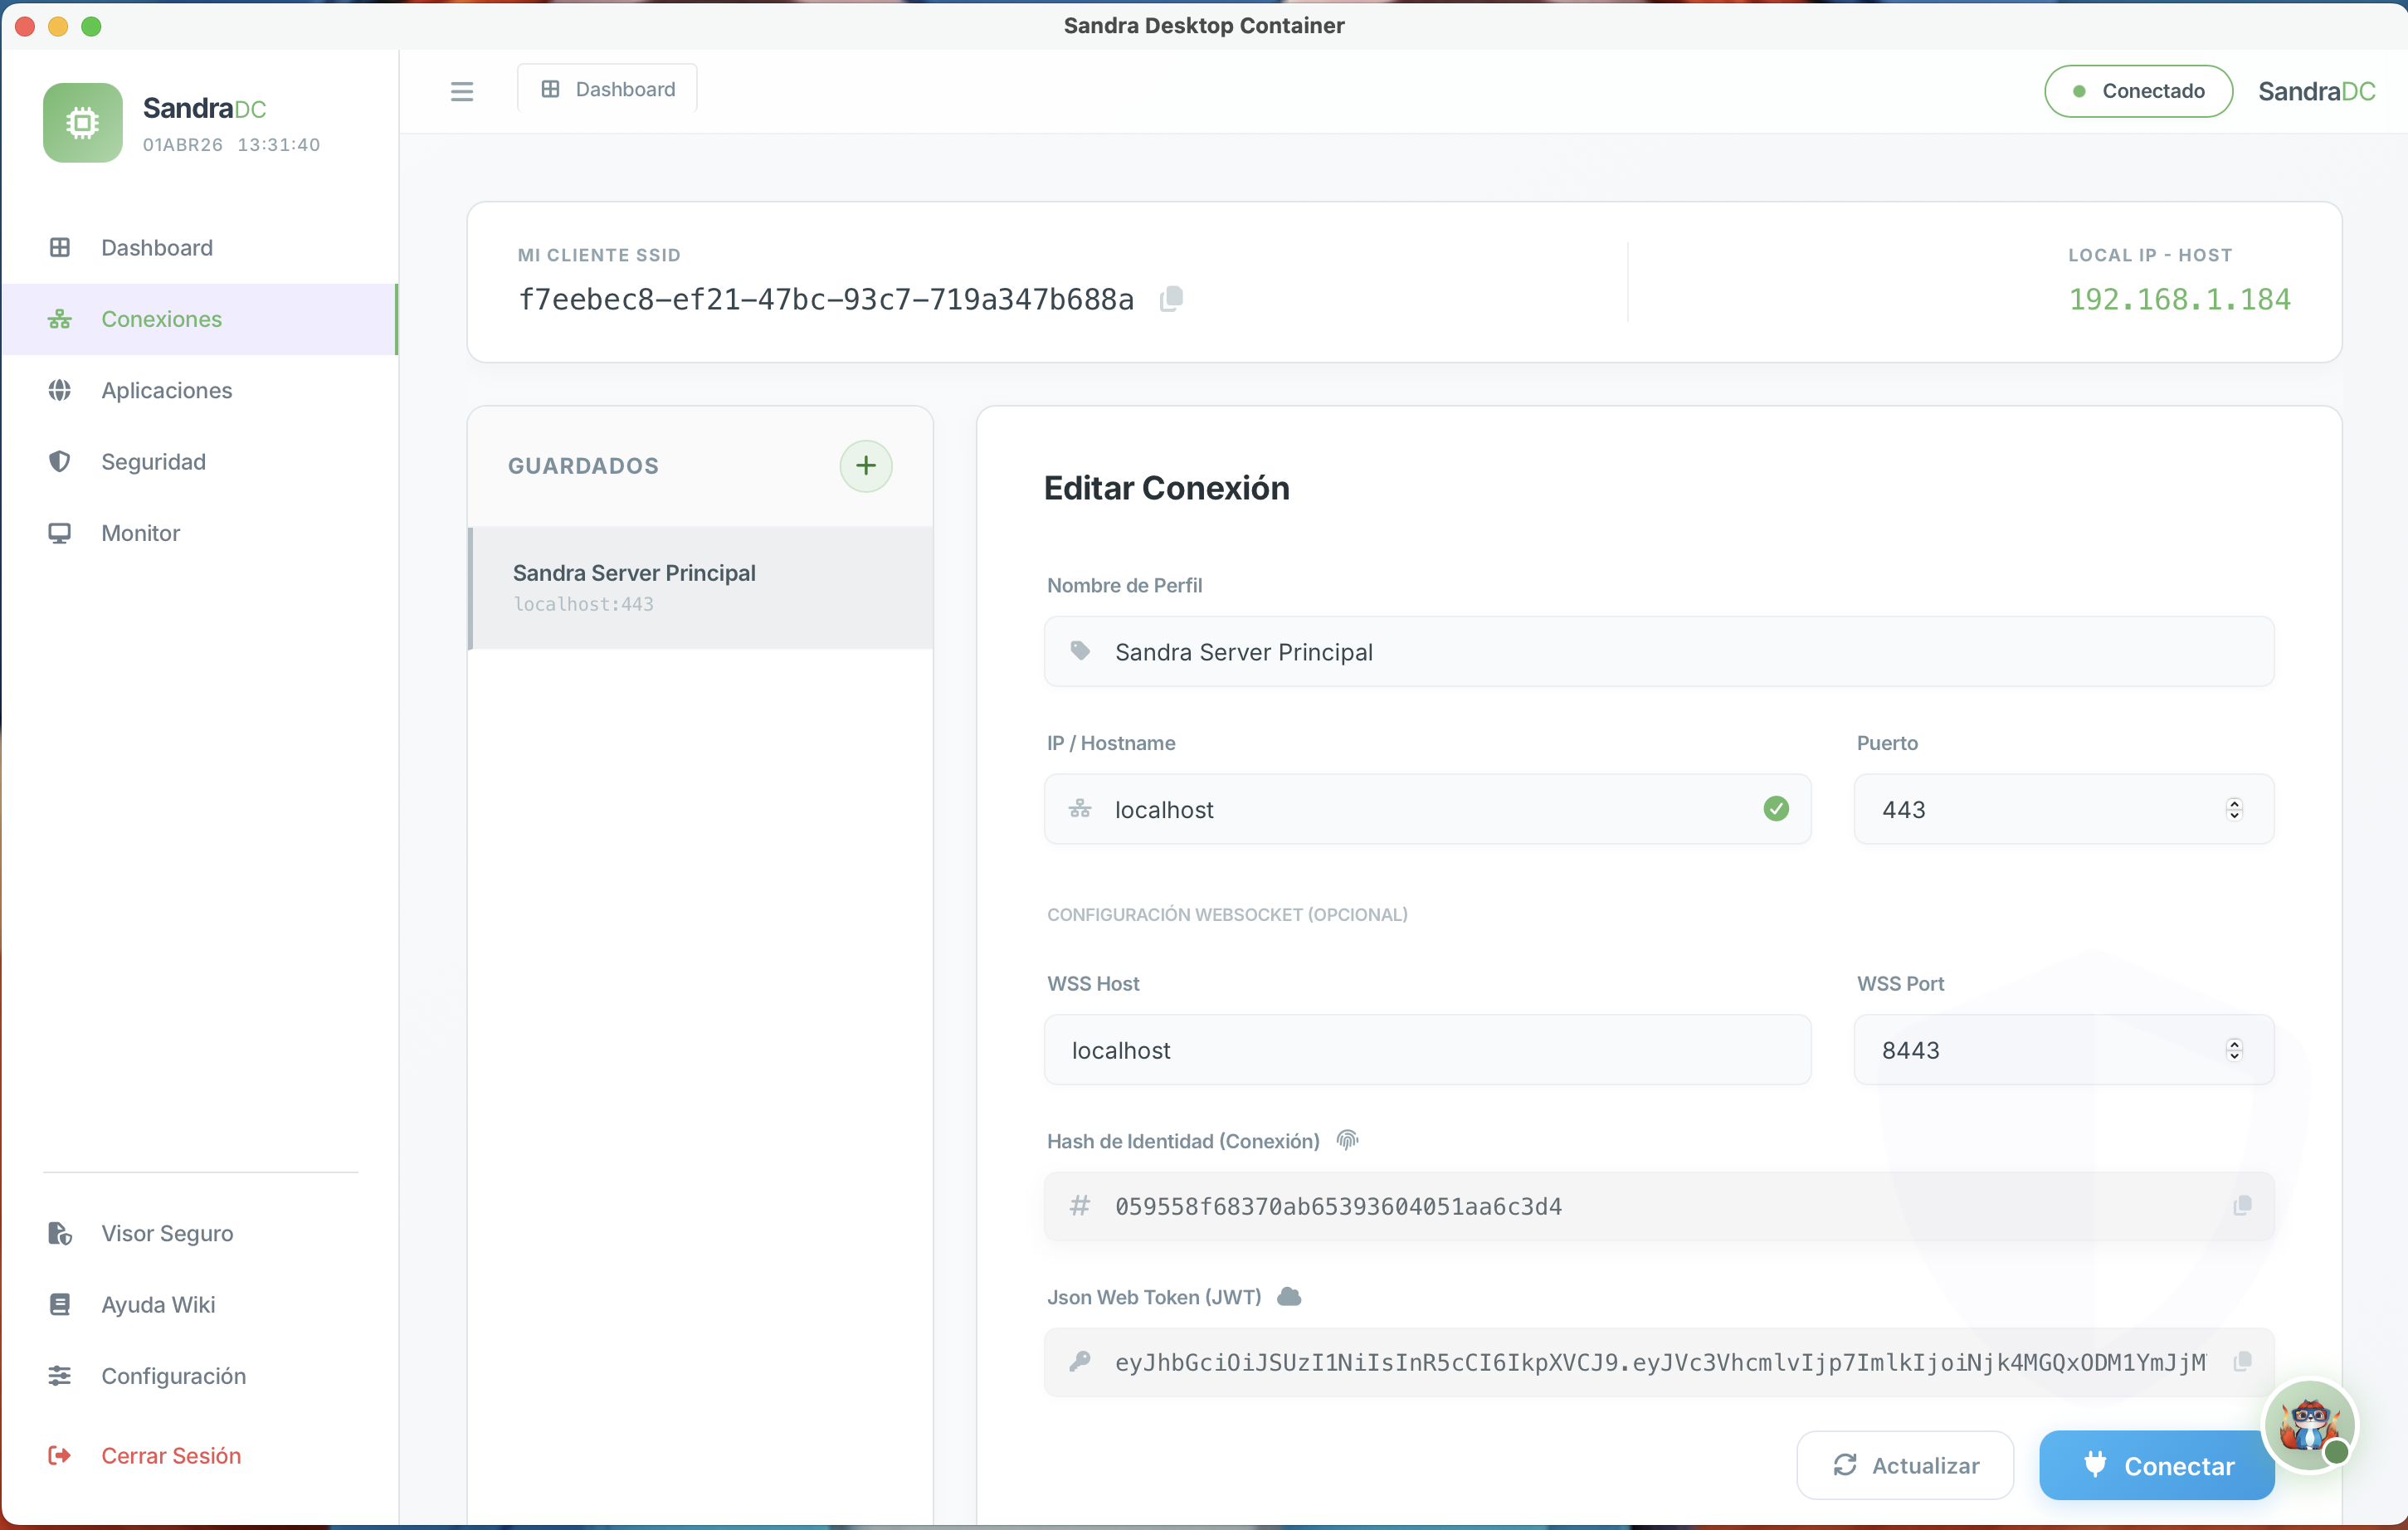
\includegraphics[width=0.95\textwidth]{anexos/5 conexion.png}
\caption{Interfaz de gestion de conexiones}
\label{fig:conexiones}
\end{figure}

\subsection{Creacion de Nueva Conexion}

Para establecer una nueva conexion a un servidor:

\begin{enumerate}[leftmargin=*]
    \item En el dashboard, hacer clic en Nueva Conexion
    \item Completar el formulario de configuracion basica
    \item Configurar opciones de seguridad (recomendado: WSS)
    \item Probar la conexion antes de guardar
    \item Asignar un nombre descriptivo al perfil
\end{enumerate}

\subsection{Parametros de Conexion}

\begin{table}[H]
\centering
\begin{tabular}{p{4cm}p{3cm}p{6cm}}
\toprule
\textbf{Parametro} & \textbf{Ejemplo} & \textbf{Descripcion} \\
\midrule
Host & servidor.com & Direccion IP o dominio \\
Puerto & 8443 & Puerto de escucha \\
Protocolo & WSS / WS & WebSocket Secure o WebSocket plano \\
Nombre & Produccion & Identificador del perfil \\
\bottomrule
\end{tabular}
\caption{Parametros de configuracion de conexion}
\label{tab:parametros-conexion}
\end{table}

\begin{quote}
\textbf{Seguridad de Conexiones}\\
Se recomienda utilizar siempre WSS (WebSocket Secure) en el puerto 8443 o superior. Las conexiones WS (sin cifrar) solo deben usarse en entornos de desarrollo controlados.
\end{quote}

\section{Gestion de Aplicaciones}
\label{sec:aplicaciones}

SDC permite convertir servicios web en aplicaciones de escritorio independientes mediante el contenedor seguro. La gestion de aplicaciones se divide en dos vistas principales: la lista de aplicaciones y el formulario de configuracion.

\subsection{Lista de Aplicaciones}
\label{subsec:lista-apps}

La vista principal muestra todas las aplicaciones disponibles y desplegadas en el sistema.

\begin{figure}[H]
\centering
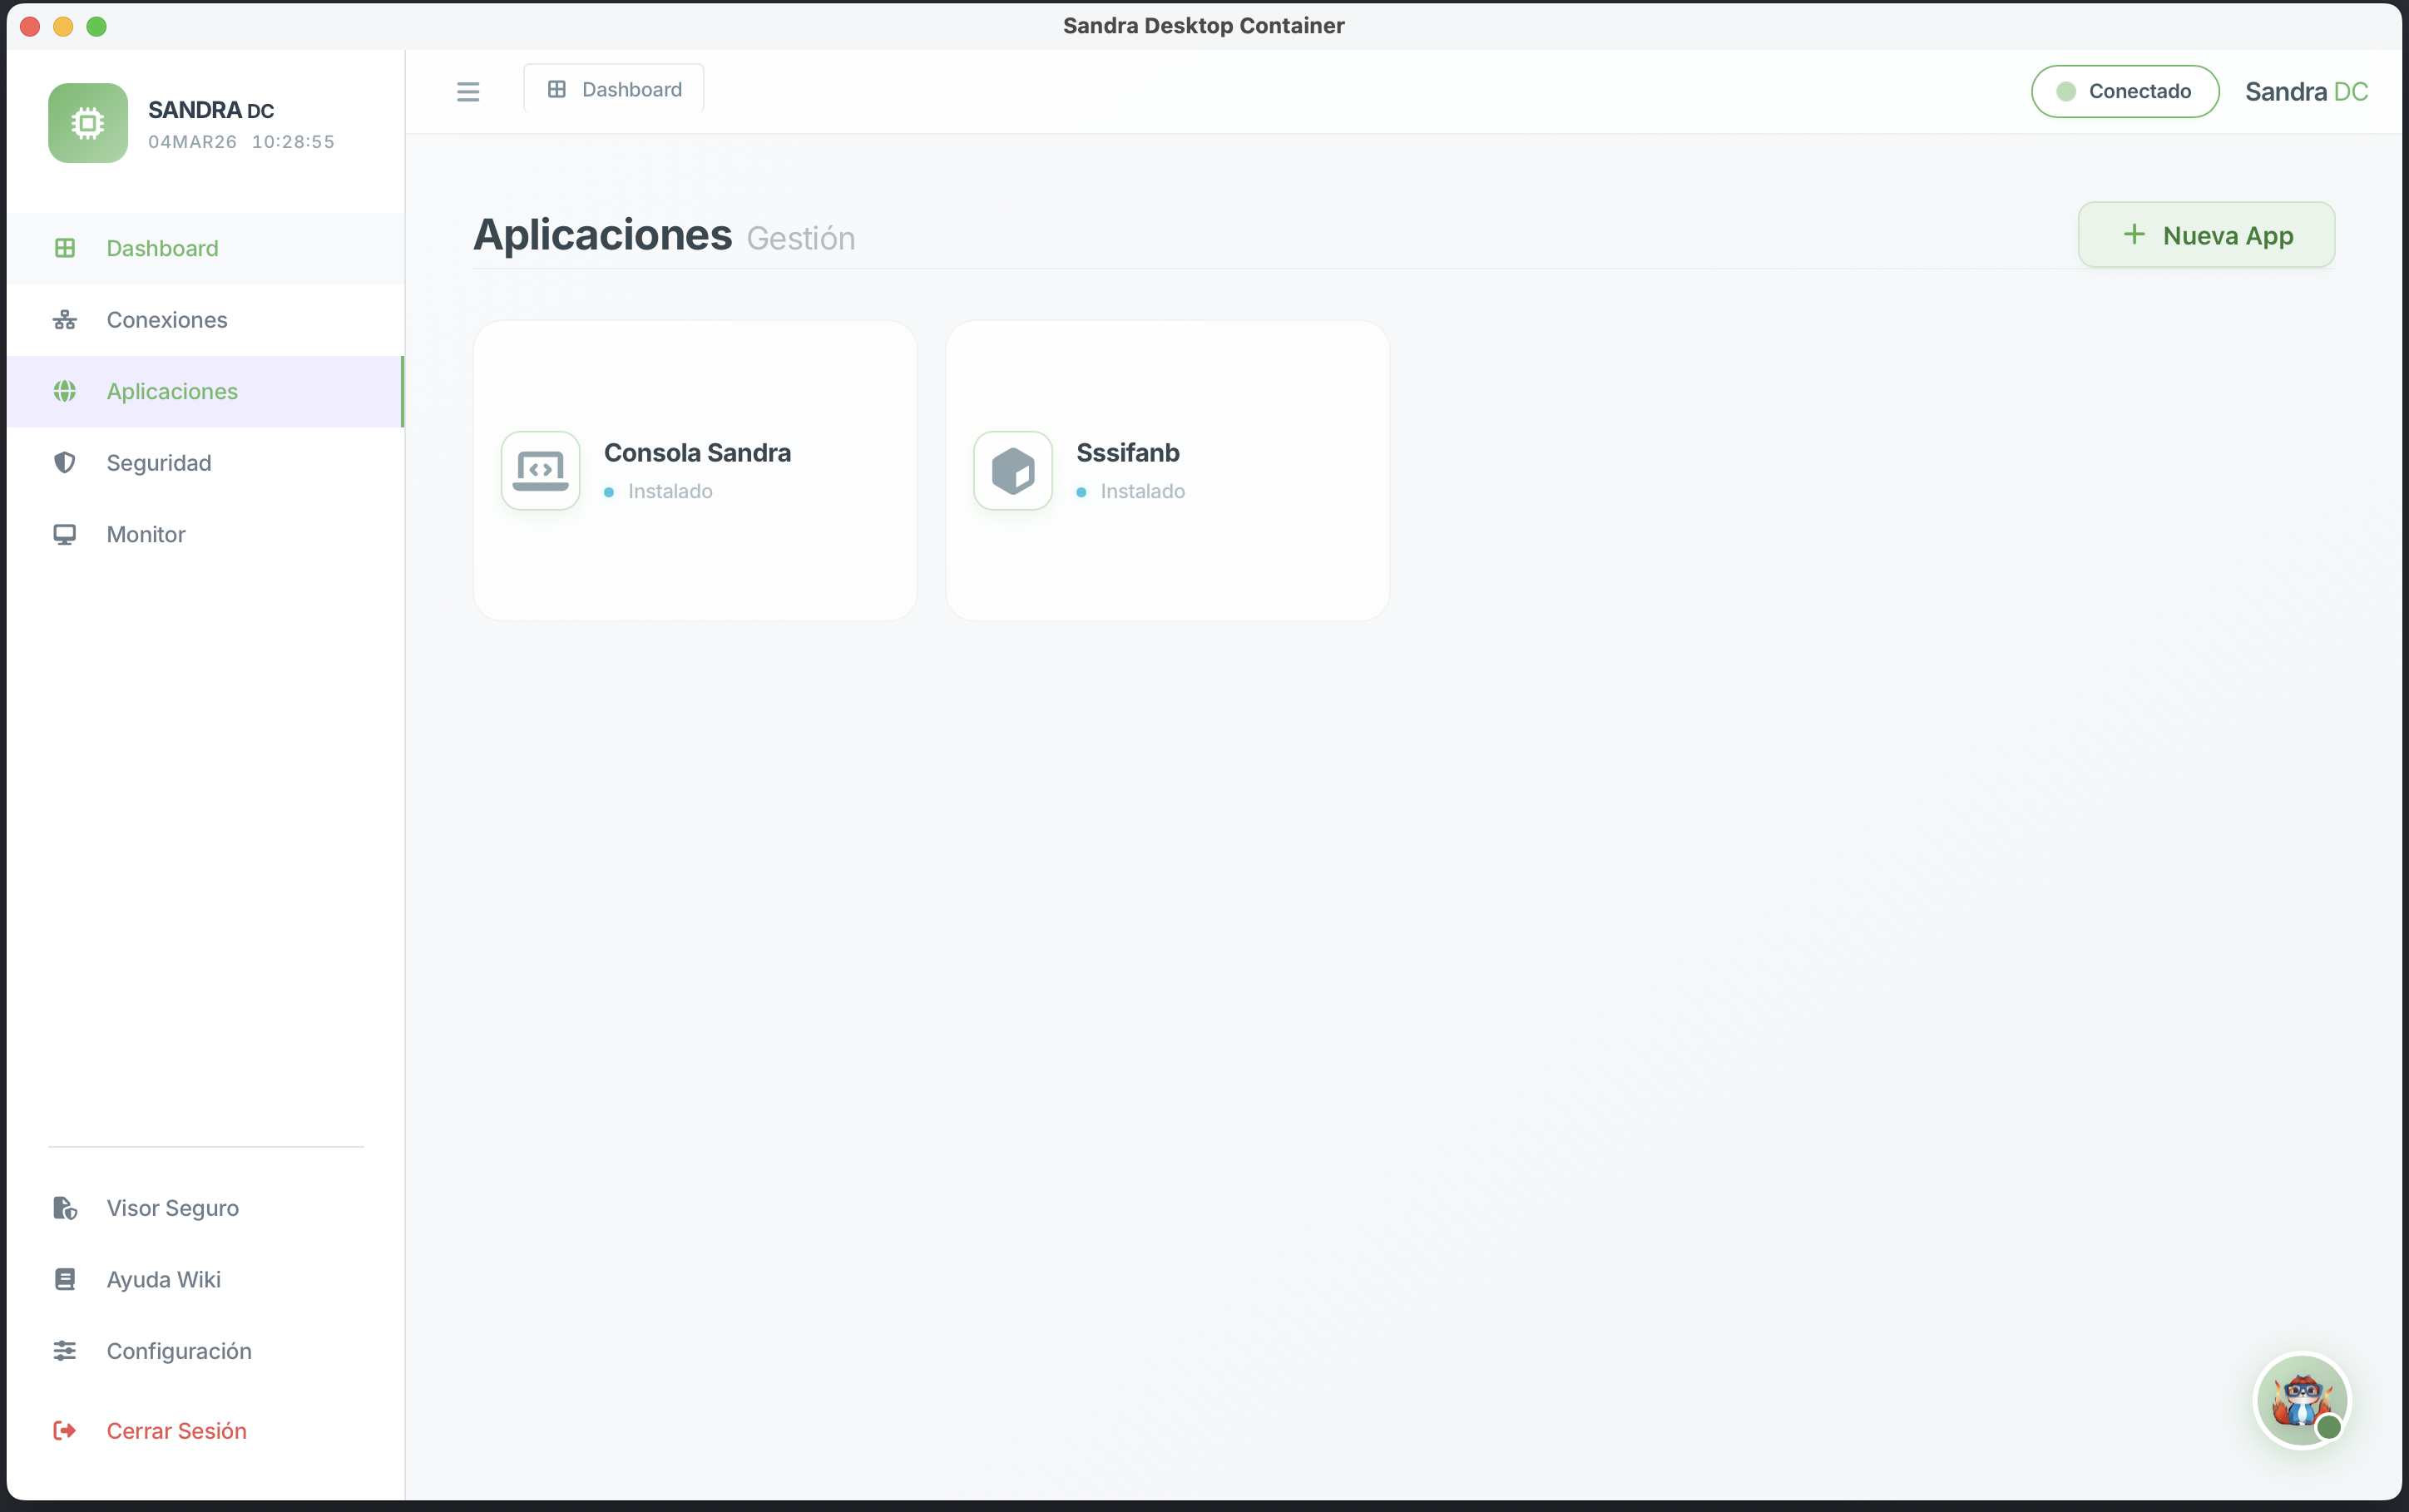
\includegraphics[width=0.95\textwidth]{anexos/6 aplicaciones.png}
\caption{Lista de aplicaciones disponibles e instaladas}
\label{fig:lista-apps}
\end{figure}

La interfaz de lista muestra:

\begin{itemize}[leftmargin=*]
    \item \textbf{Aplicaciones Instaladas}: Apps desplegadas y listas para usar
    \item \textbf{Aplicaciones Disponibles}: Catalogo de apps que pueden instalarse
    \item \textbf{Indicadores de Estado}: Iconos que muestran si esta activa, proxy requerido, o modo libre
    \item \textbf{Acciones Rapidas}: Botones para abrir, actualizar o desactivar cada app
\end{itemize}

\begin{quote}
\textbf{Indicadores Visuales}
\begin{itemize}
    \item Punto verde: Aplicacion instalada y activa
    \item Punto gris: Aplicacion disponible pero no instalada
    \item Icono \texttt{fa-shield-alt}: Requiere proxy seguro
    \item Icono \texttt{fa-globe-americas}: Modo navegacion libre
\end{itemize}
\end{quote}

\subsection{Formulario de Nueva Aplicacion}
\label{subsec:formulario-apps}

Al instalar o configurar una aplicacion, se accede al formulario completo de configuracion.

\begin{figure}[H]
\centering
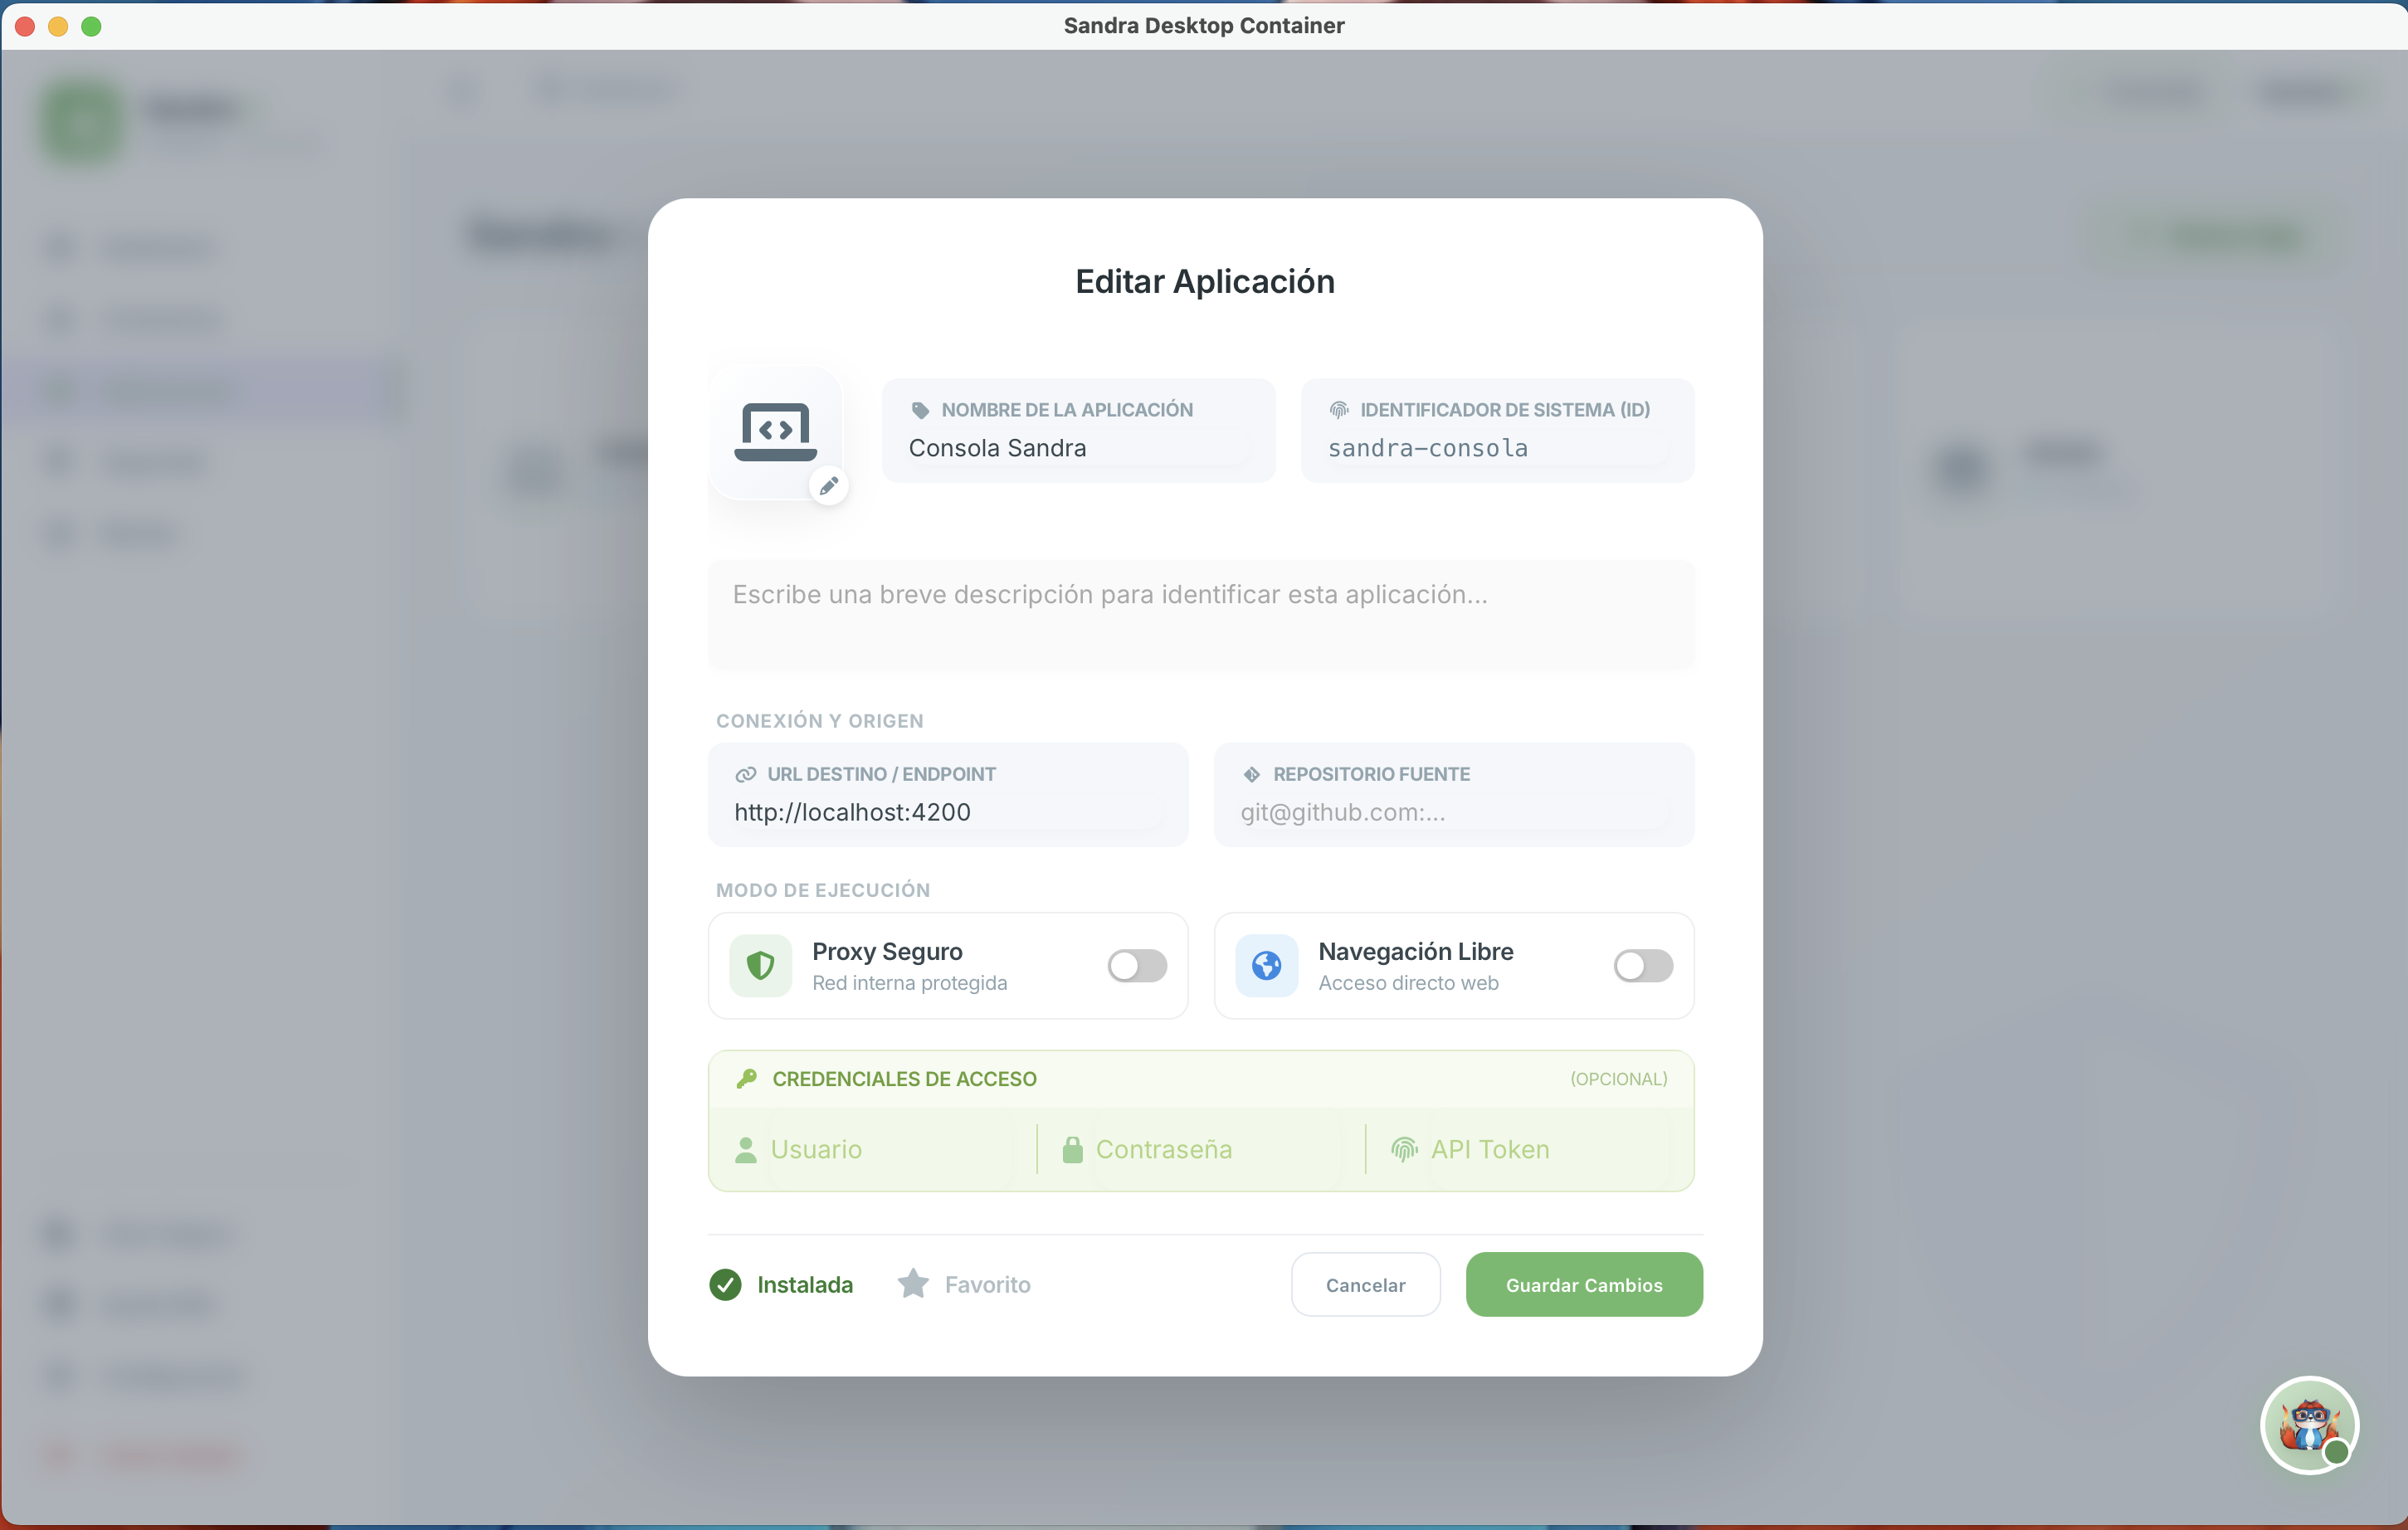
\includegraphics[width=0.95\textwidth]{anexos/6 aplicaciones nueva.png}
\caption{Formulario completo de creacion de aplicacion}
\label{fig:formulario-apps}
\end{figure}

\subsubsection{Campos de Configuracion}

\begin{table}[H]
\centering
\begin{tabular}{p{4cm}p{3cm}p{6cm}}
\toprule
\textbf{Campo} & \textbf{Requerido} & \textbf{Descripcion} \\
\midrule
Nombre & Si & Identificador de la aplicacion \\
URL & Si & Direccion del servicio web \\
Modo de Proxy & Si & Seguro o Navegacion Libre \\
Repositorio & No & URL de Git para actualizaciones \\
Icono & No & Imagen personalizada (256x256) \\
\bottomrule
\end{tabular}
\caption{Campos del formulario de aplicacion}
\label{tab:campos-apps}
\end{table}

\subsubsection{Modos de Despliegue}

\begin{table}[H]
\centering
\begin{tabular}{p{4cm}p{9cm}}
\toprule
\textbf{Modo} & \textbf{Descripcion} \\
\midrule
\textbf{Proxy Seguro} & Enmascara la IP real mediante tuneles cifrados. Todo el trafico se enruta a traves de WSS con autenticacion de cliente. Ideal para aplicaciones criticas y datos sensibles. \\
\midrule
\textbf{Navegacion Libre} & Acceso directo sin tuneles adicionales. El trafico fluye directamente entre cliente y servidor. Para aplicaciones internas de baja criticidad o desarrollo. \\
\bottomrule
\end{tabular}
\caption{Modos de despliegue de aplicaciones}
\label{tab:modos-despliegue}
\end{table}

\subsection{Repositorio Fuente}

SDC permite vincular aplicaciones a repositorios de codigo:

\begin{lstlisting}[language=bash, caption={Configuracion de Repositorio}]
# Soporte para:
- GitHub (github.com/usuario/repo)
- GitLab (gitlab.com/usuario/repo)
- Bitbucket (bitbucket.org/usuario/repo)
- Repositorio privado (URL + credenciales)

# Opciones de despliegue automatico:
- Actualizar al iniciar
- Actualizar manualmente
- Actualizar programada (cron)
\end{lstlisting}

\begin{quote}
\textbf{Despliegue Automatico}\\
Cuando se activa, SDC verifica cambios cada 5 minutos y notifica al usuario cuando hay nueva version disponible.
\end{quote}

\section{Lista de Conexiones Activas}
\label{sec:conexiones-activas}

El panel de conexiones activas permite monitorear todas las conexiones establecidas.

\begin{figure}[H]
\centering
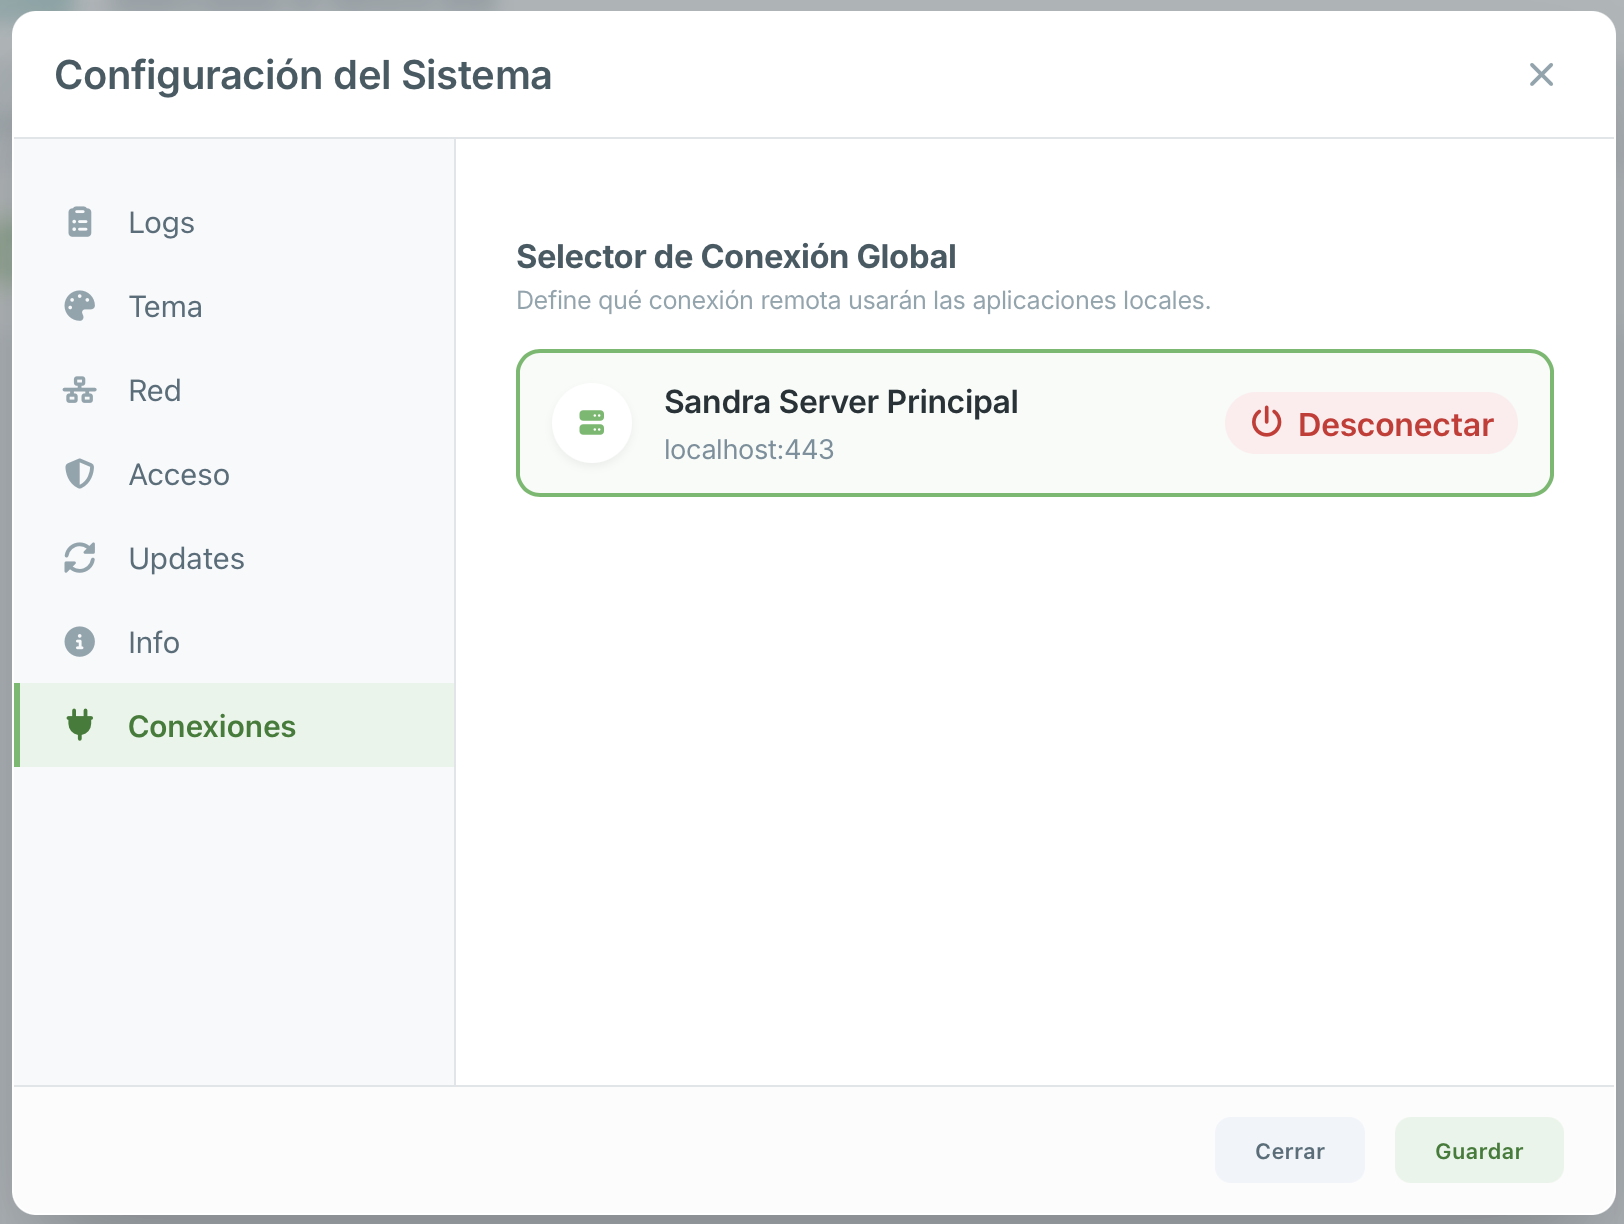
\includegraphics[width=0.95\textwidth]{anexos/16 conexiones activas.png}
\caption{Monitor de conexiones activas}
\label{fig:conexiones-activas}
\end{figure}

\subsection{Informacion Visualizada}

Para cada conexion activa, el sistema muestra:

\begin{itemize}[leftmargin=*]
    \item Estado (Verde: Activa, Rojo: Error, Gris: Inactiva)
    \item Nombre del perfil de conexion
    \item Host y puerto destino
    \item Tiempo de actividad (uptime)
    \item Latencia actual en ms
    \item Bytes transferidos
\end{itemize}

\section{Gestion del Monitor del Sistema}
\label{sec:monitor}

El modulo de monitoreo proporciona metricas detalladas de bajo nivel.

\begin{figure}[H]
\centering
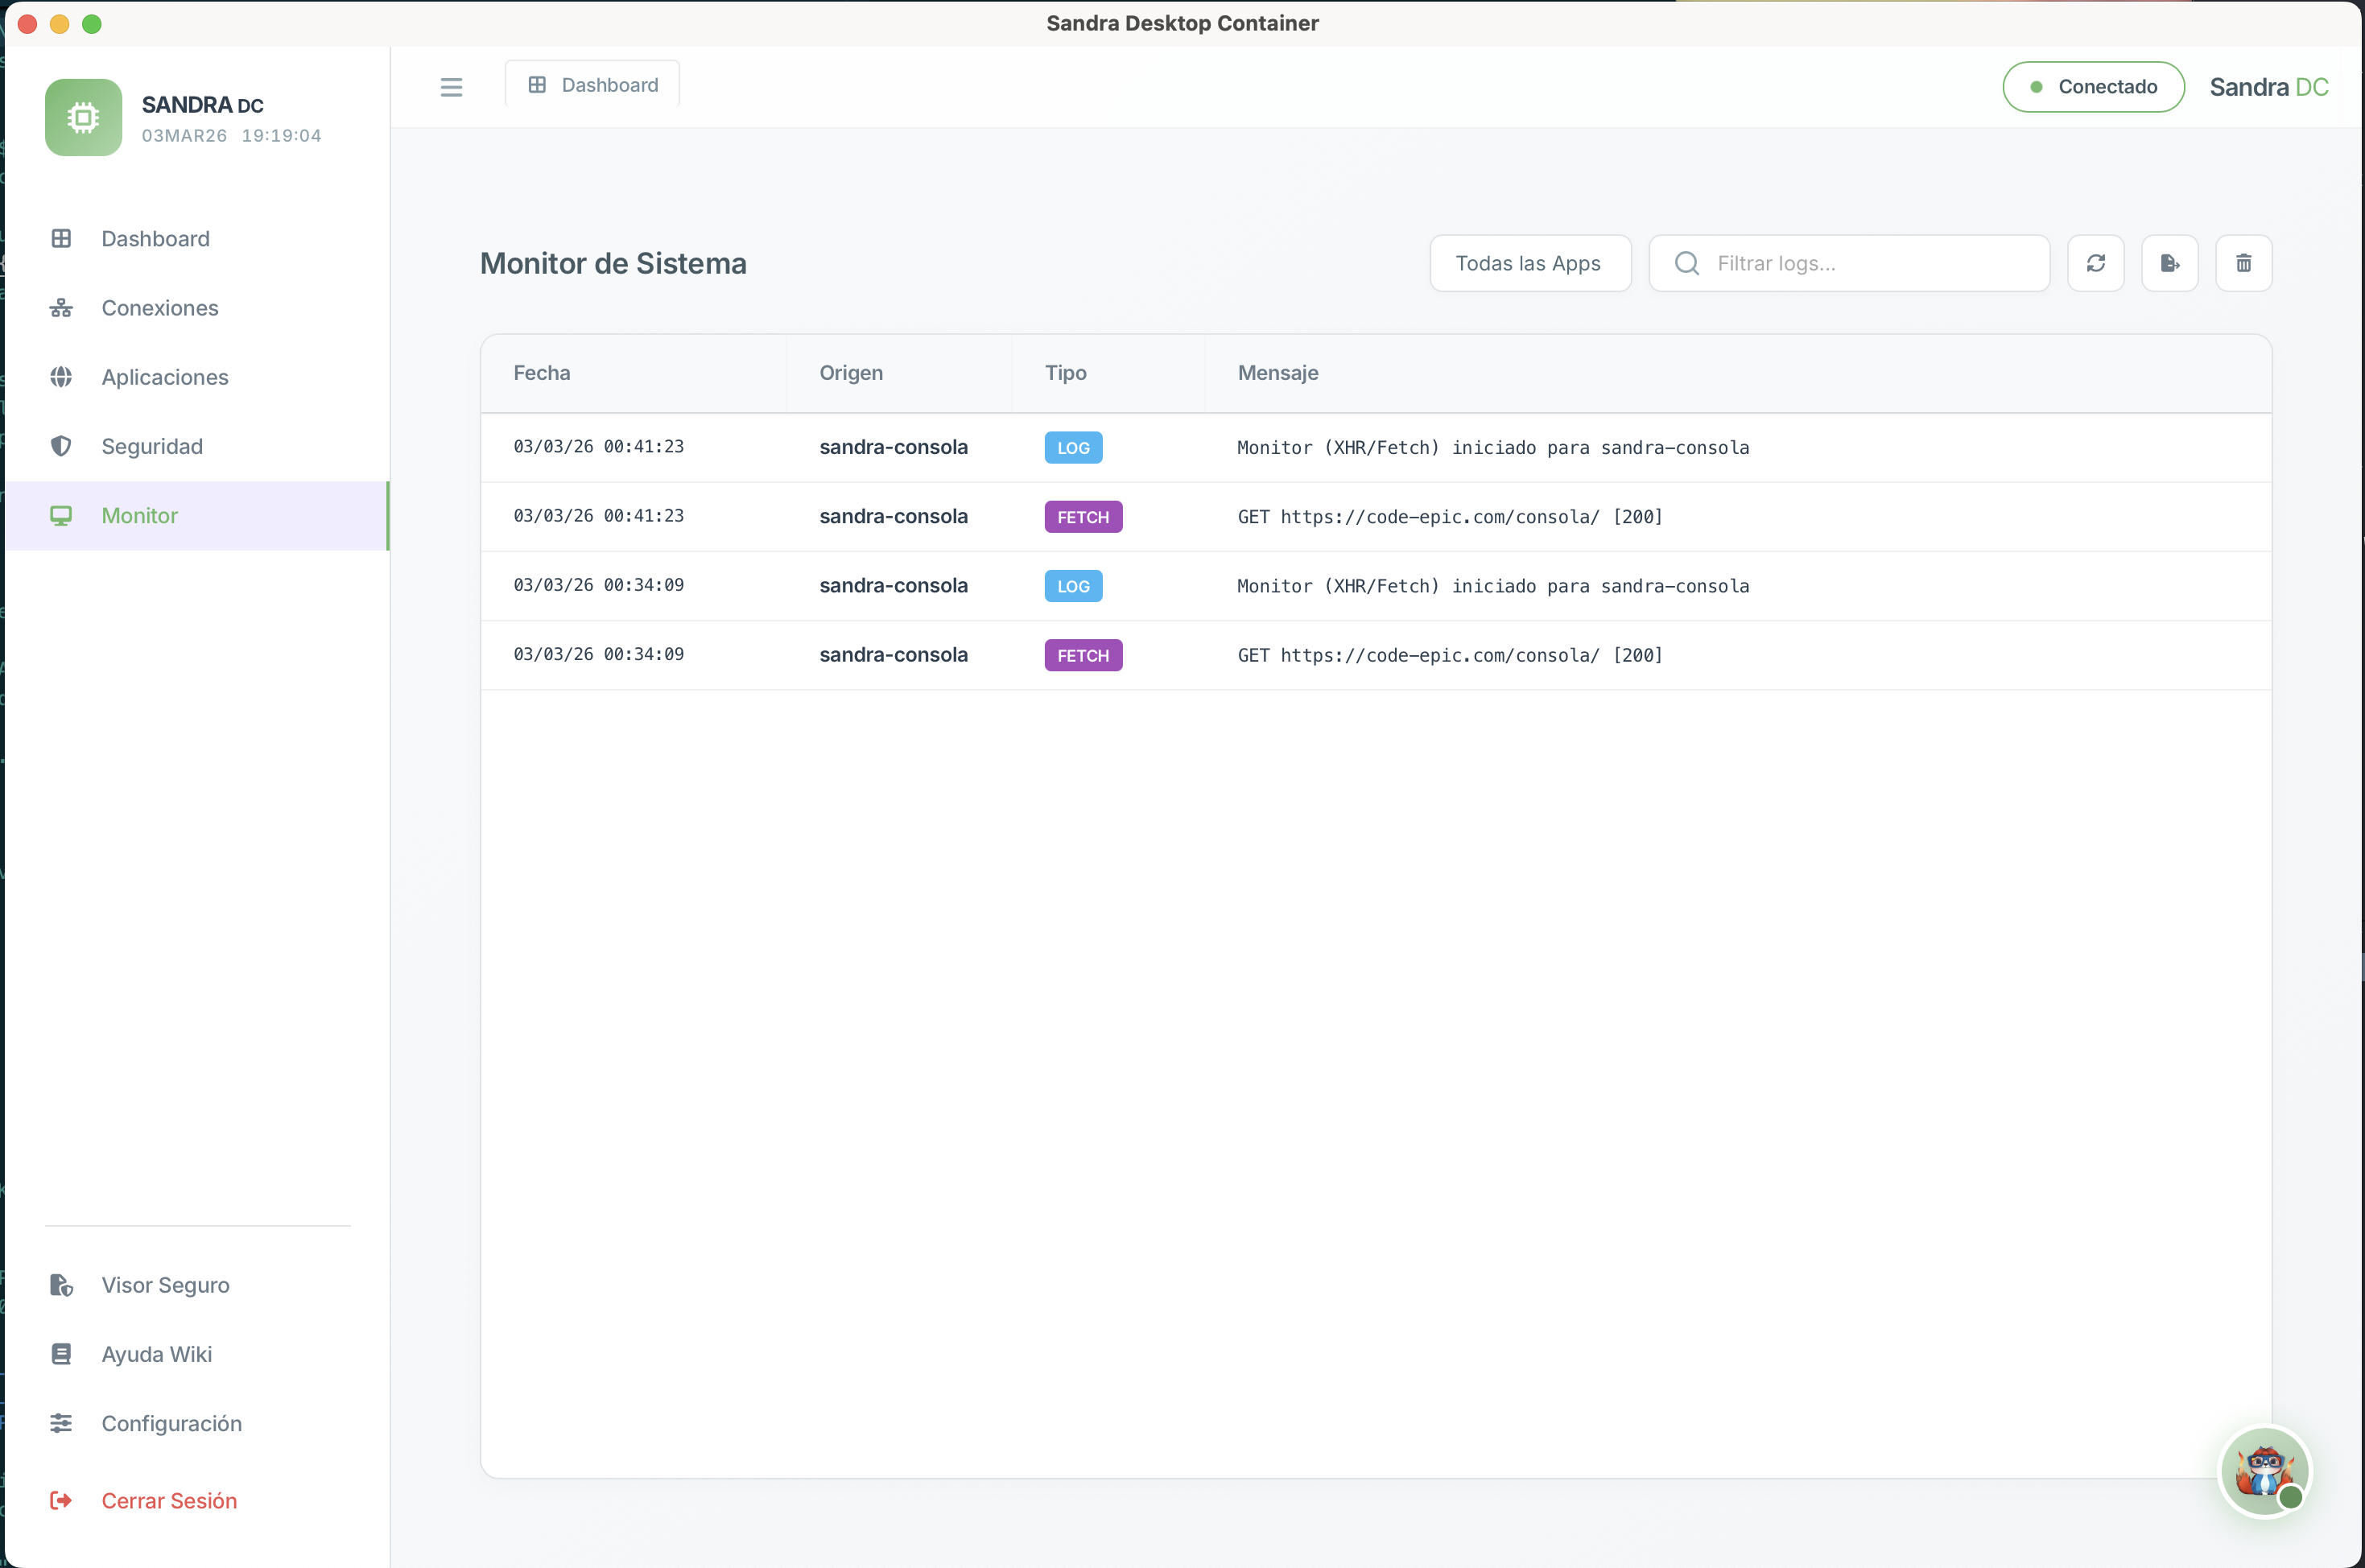
\includegraphics[width=0.95\textwidth]{anexos/10 monitor.png}
\caption{Monitor del sistema en tiempo real}
\label{fig:monitor}
\end{figure}

\subsection{Metricas de Hardware}

\begin{table}[H]
\centering
\begin{tabular}{p{3cm}p{5cm}p{5cm}}
\toprule
\textbf{Recurso} & \textbf{Metrica} & \textbf{Umbral de Alerta} \\
\midrule
CPU & Uso porcentual por nucleo & Mayor a 90 por ciento sostenido \\
RAM & Uso en GB / Total disponible & Mayor a 85 por ciento uso \\
Red & Paquetes/s y bytes/s & Latencia mayor a 500ms \\
Disco & I/O operaciones por segundo & Tiempo mayor a 100ms \\
\bottomrule
\end{tabular}
\caption{Metricas monitoreadas del sistema}
\label{tab:metricas-monitor}
\end{table}

\subsection{Inspector de Red}

Herramienta de transparencia que permite auditar el trafico de red:

\begin{itemize}[leftmargin=*]
    \item Interceptacion pasiva de peticiones Fetch/XHR
    \item Visualizacion de headers y payloads
    \item Filtrado por dominio, metodo HTTP o tipo de contenido
    \item Exportacion de logs para analisis forense
\end{itemize}

\begin{quote}
\textbf{Interceptacion Licita}\\
El Inspector de Red actua como herramienta de transparencia para auditores de seguridad. Su funcionamiento esta limitado al trafico generado por aplicaciones SDC.
\end{quote}

\section{Buzon de Seguridad (Mailbox)}
\label{sec:mailbox}

El modulo de \keyconcept{Buzon de Seguridad} es el corazon de la persistencia y comunicacion asincrona del contenedor. Diseñado para cumplir con estandares de alta disponibilidad y seguridad criptografica avanzada.

\notacientifica{El Buzon de Seguridad (Mailbox) implementa una arquitectura desacoplada que garantiza mantenibilidad, testabilidad y rendimiento optimo en entornos de produccion.}

\subsection{Arquitectura del Mailbox}

El modulo se organiza siguiendo patrones de diseño establecidos:

\begin{caja}{Patrones de Arquitectura}
\begin{itemize}
\item \textbf{Patron Repository}: Toda la persistencia en SQLite se centraliza en MailboxRepository, eliminando la dispersion de SQL en los controladores de Tauri. Maneja transacciones atomicas para asegurar la integridad de los datos.

\item \textbf{Sync Service}: Gestiona la orquestacion entre la API remota (Sandra Server) y la base de datos local.

\item \textbf{Streaming NDJSON}: El procesamiento de mensajes entrantes utiliza un buffer de streaming que analiza lineas NDJSON (Newline Delimited JSON) al vuelo, permitiendo procesar miles de mensajes sin picos de consumo de memoria RAM.
\end{itemize}
\end{caja}

\notacientifica{La arquitectura separada permite que cada componente evolucione de manera independiente sin afectar a los demas.}

\subsection{Optimizacion de Rendimiento}

Para manejar volumenes de datos masivos (mas de 1000 mensajes) sin degradar la experiencia de usuario, SDC implementa sincronizacion industrial:

\begin{caja}{Tecnicas de Optimizacion}
\begin{itemize}
\item \textbf{NDJSON Streaming}: La sincronizacion de buzon utiliza una arquitectura de flujo continuo que procesa cada mensaje en milisegundos conforme llega del servidor, evitando la carga masiva de objetos en el heap de JavaScript.

\item \textbf{Deduplicacion Predictiva}: Uso de un Set de GUIDs (Global Unique Identifiers) en memoria para filtrar instantaneamente mensajes que ya residen en la base de datos local, ahorrando ciclos de escritura en disco.

\item \textbf{ACK Segmentado y Flushing}: El sistema envia confirmaciones de recepcion (ACK) en lotes mediante streaming, permitiendo que el servidor libere los mensajes del nodo de origen de forma eficiente.

\item \textbf{Background Sync Logic}: La sincronizacion de mensajes ocurre en hilos paralelos de Rust, mientras la UI en Angular se mantiene fluida y reactiva.
\end{itemize}
\end{caja}

\notacientifica{Estas tecnicas permiten manejar miles de mensajes por segundo sin degradar la interfaz de usuario.}

\subsection{Certificacion Automatica de Descarga}

Cada mensaje que ingresa al contenedor es procesado por un motor de certificacion que garantiza su trazabilidad:

\begin{caja}{Proceso de Certificacion}
\begin{enumerate}
\item \textbf{ACK Automatico}: El sistema confirma al servidor la recepcion exitosa para limpiar colas de alta fidelidad.
\item \textbf{Tag de Auditoria}: Se inyecta un estado de "Descargado" en el mani\-esto local del mensaje para auditorias posteriores de sincronizacion completa.
\end{enumerate}
\end{caja}

\notacientifica{La certificacion automatica garantiza un registro completo de todos los mensajes, facilitando auditorias y cumplimiento normativo.}

\subsection{Modelo de Seguridad del Mailbox}

El Buzon implementa un sistema de cifrado de triple capa para paquetes seguros:

\begin{caja}{Capas de Seguridad}
\begin{enumerate}
\item \textbf{Device Secret}: Durante el setup inicial, SDC genera una clave unica de 32 bytes aleatoria almacenada en el enclave de la base de datos. Esto elimina la predecibilidad de usar solo la direccion MAC del dispositivo.

\item \textbf{Derivacion de Clave con Argon2}: La clave de cifrado AES-256-GCM se deriva dinamicamente usando Argon2id con un Salt de sistema (PACKAGE\_SALT).

\item \textbf{Dual-Key Decryption Fallback}: Para garantizar la interoperabilidad con paquetes antiguos o generados en dispositivos externos, el motor de ingesta intenta descifrar primero con el Device Secret y, en caso de fallo, utiliza la MAC Address como respaldo automatico.
\end{enumerate}
\end{caja}

\notacientifica{Este modelo de triple capa garantiza que incluso si una capa es comprometida, los datos permanecen protegidos por las capas restantes.}

\section{Interfaz del Buzon de Seguridad}

El panel de seguridad centraliza la gestion del Buzon de Seguridad, permitiendo enviar, recibir y gestionar mensajes cifrados de manera eficiente.

\begin{figure}[H]
\centering
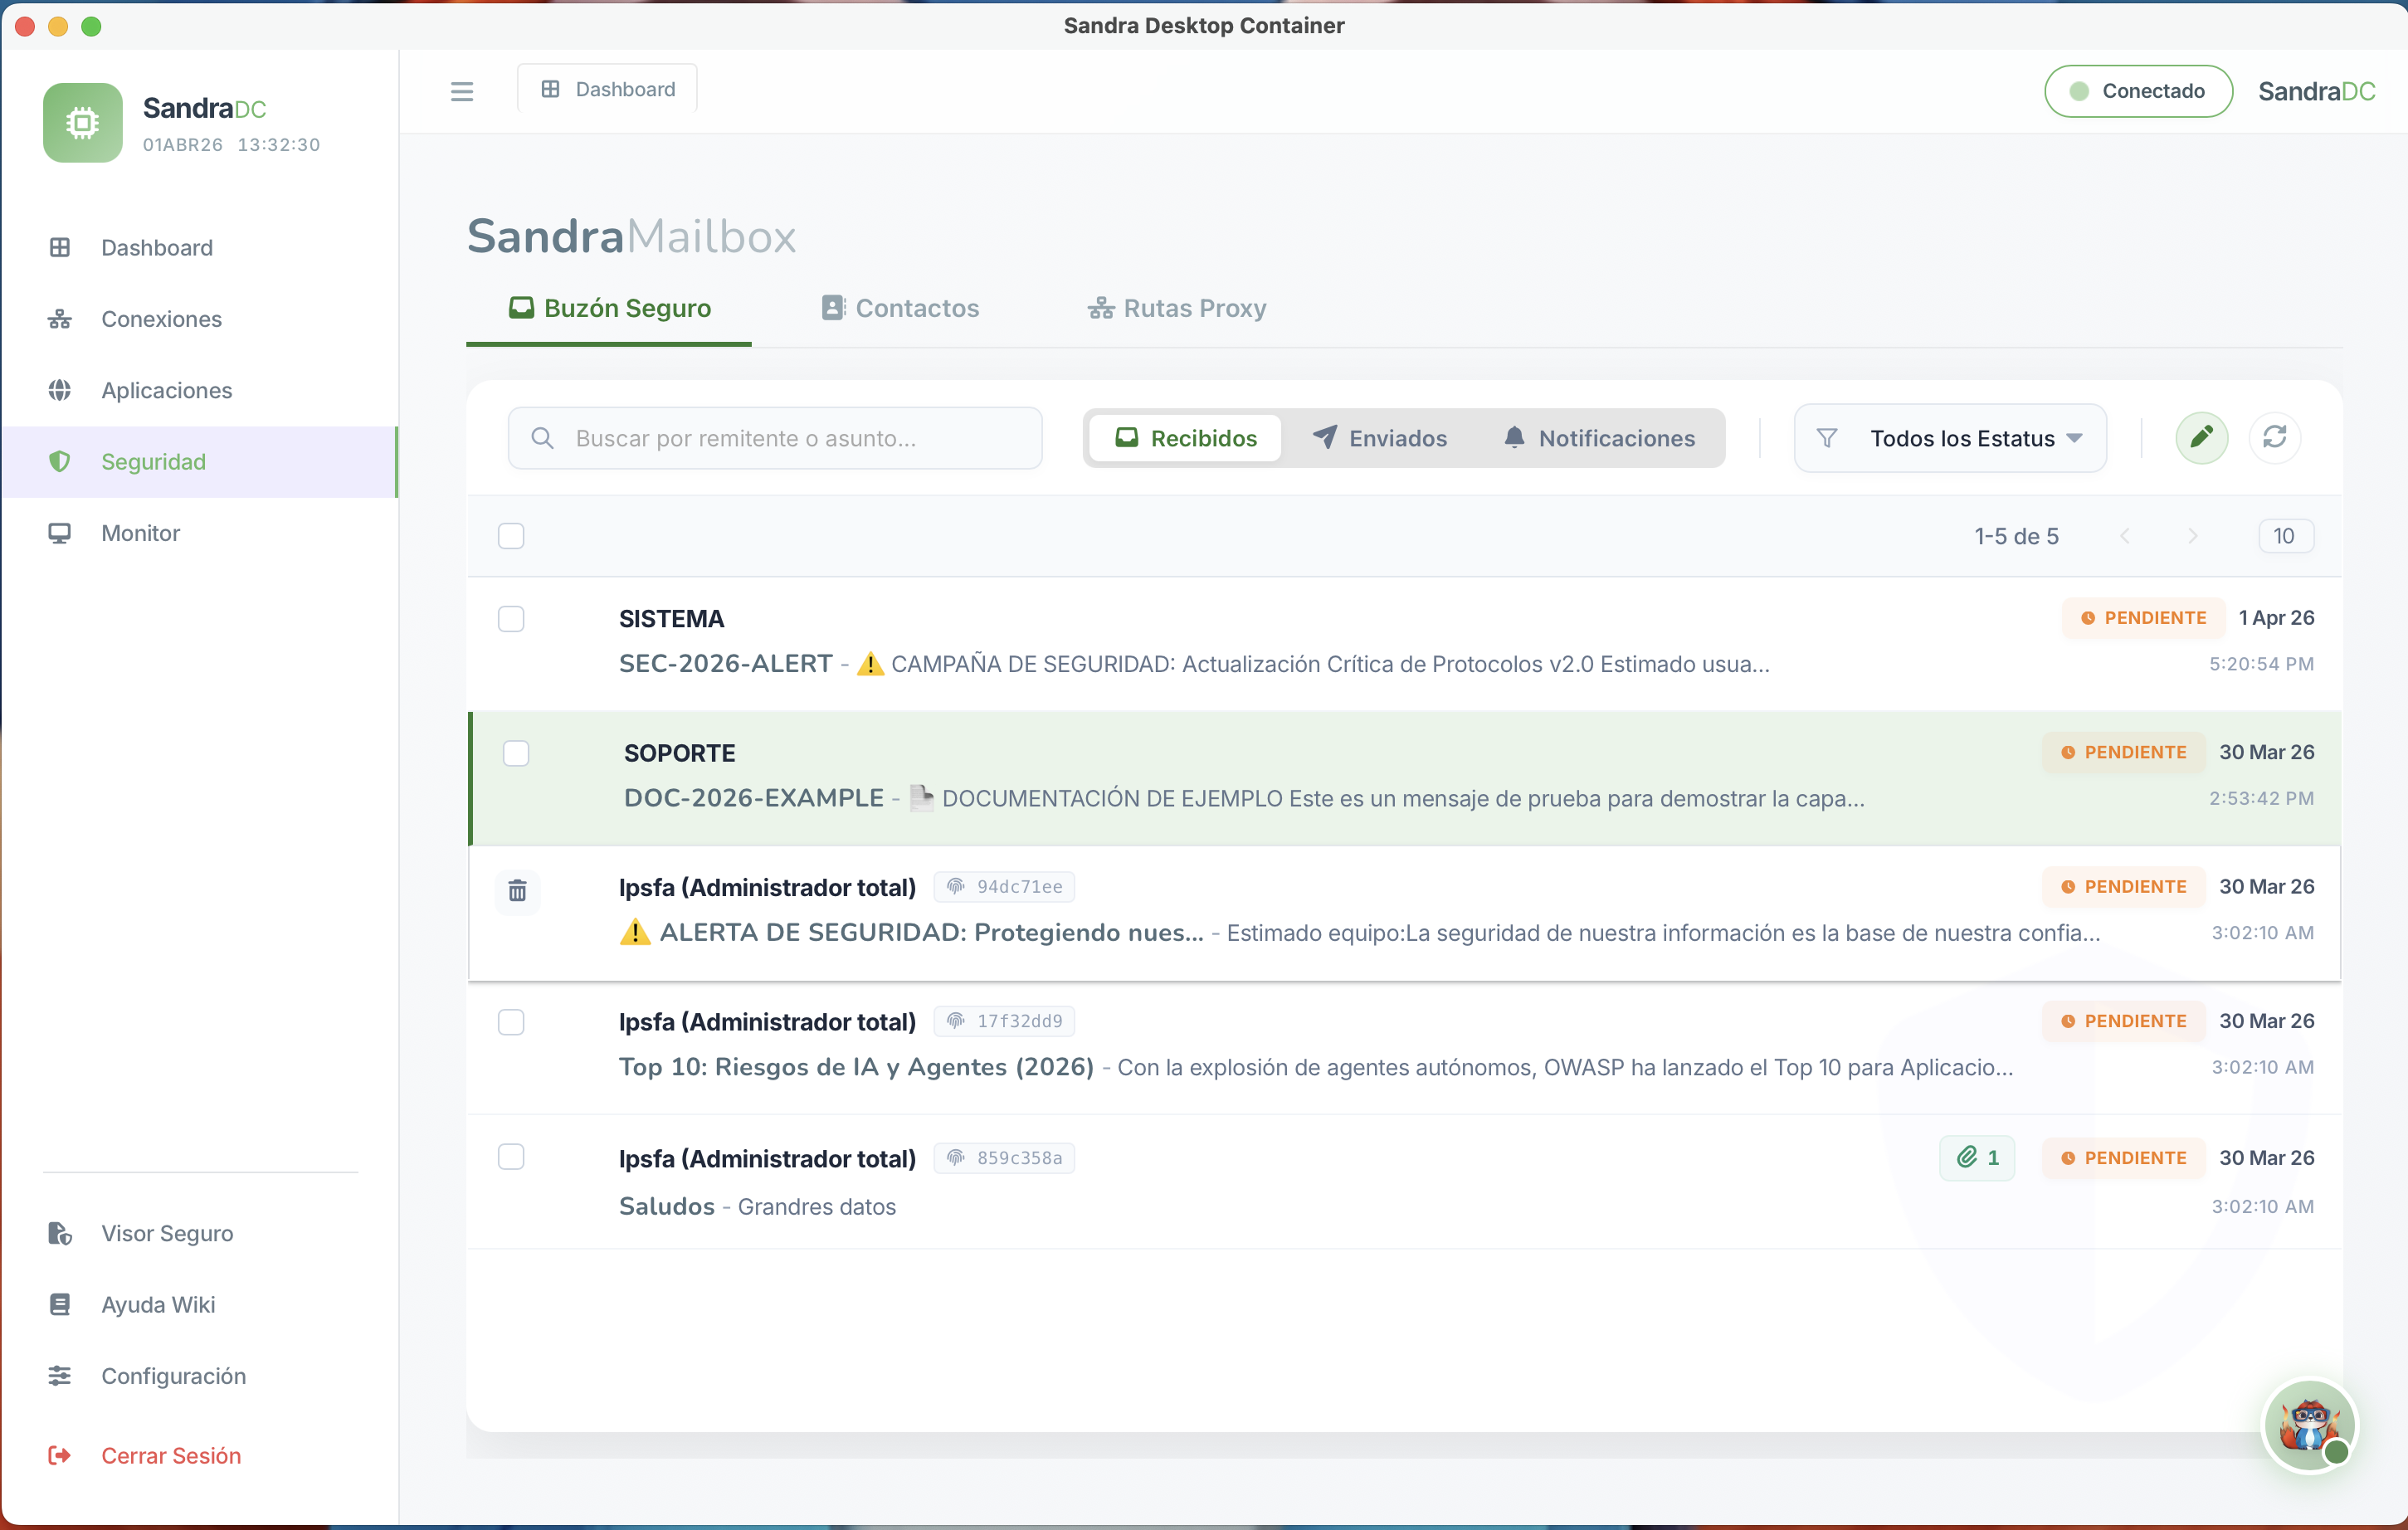
\includegraphics[width=0.95\textwidth]{anexos/7 seguridad.mailbox.png}
caption{Interfaz principal del Buzon de Seguridad}
\label{fig:mailbox-principal}
\end{figure}

\subsection{Navegacion por Pestanas}

La interfaz del Buzon de Seguridad se organiza en pestanas que permiten diferentes operaciones:

\begin{enumerate}
    \item \textbf{Bandeja de Entrada}: Mensajes recibidos y pendientes de lectura
    \item \textbf{Enviados}: Mensajes cifrados y enviados a otros usuarios
    \item \textbf{Redactar}: Composicion de nuevos mensajes seguros
    \item \textbf{Notificaciones}: Alertas del sistema y confirmaciones de entrega
\end{enumerate}

\notacientifica{Cada pestana mantiene su propio estado de sincronizacion, permitiendo trabajar offline con mensajes previamente descargados.}

\subsection{Composicion de Mensajes}

\begin{figure}[H]
\centering
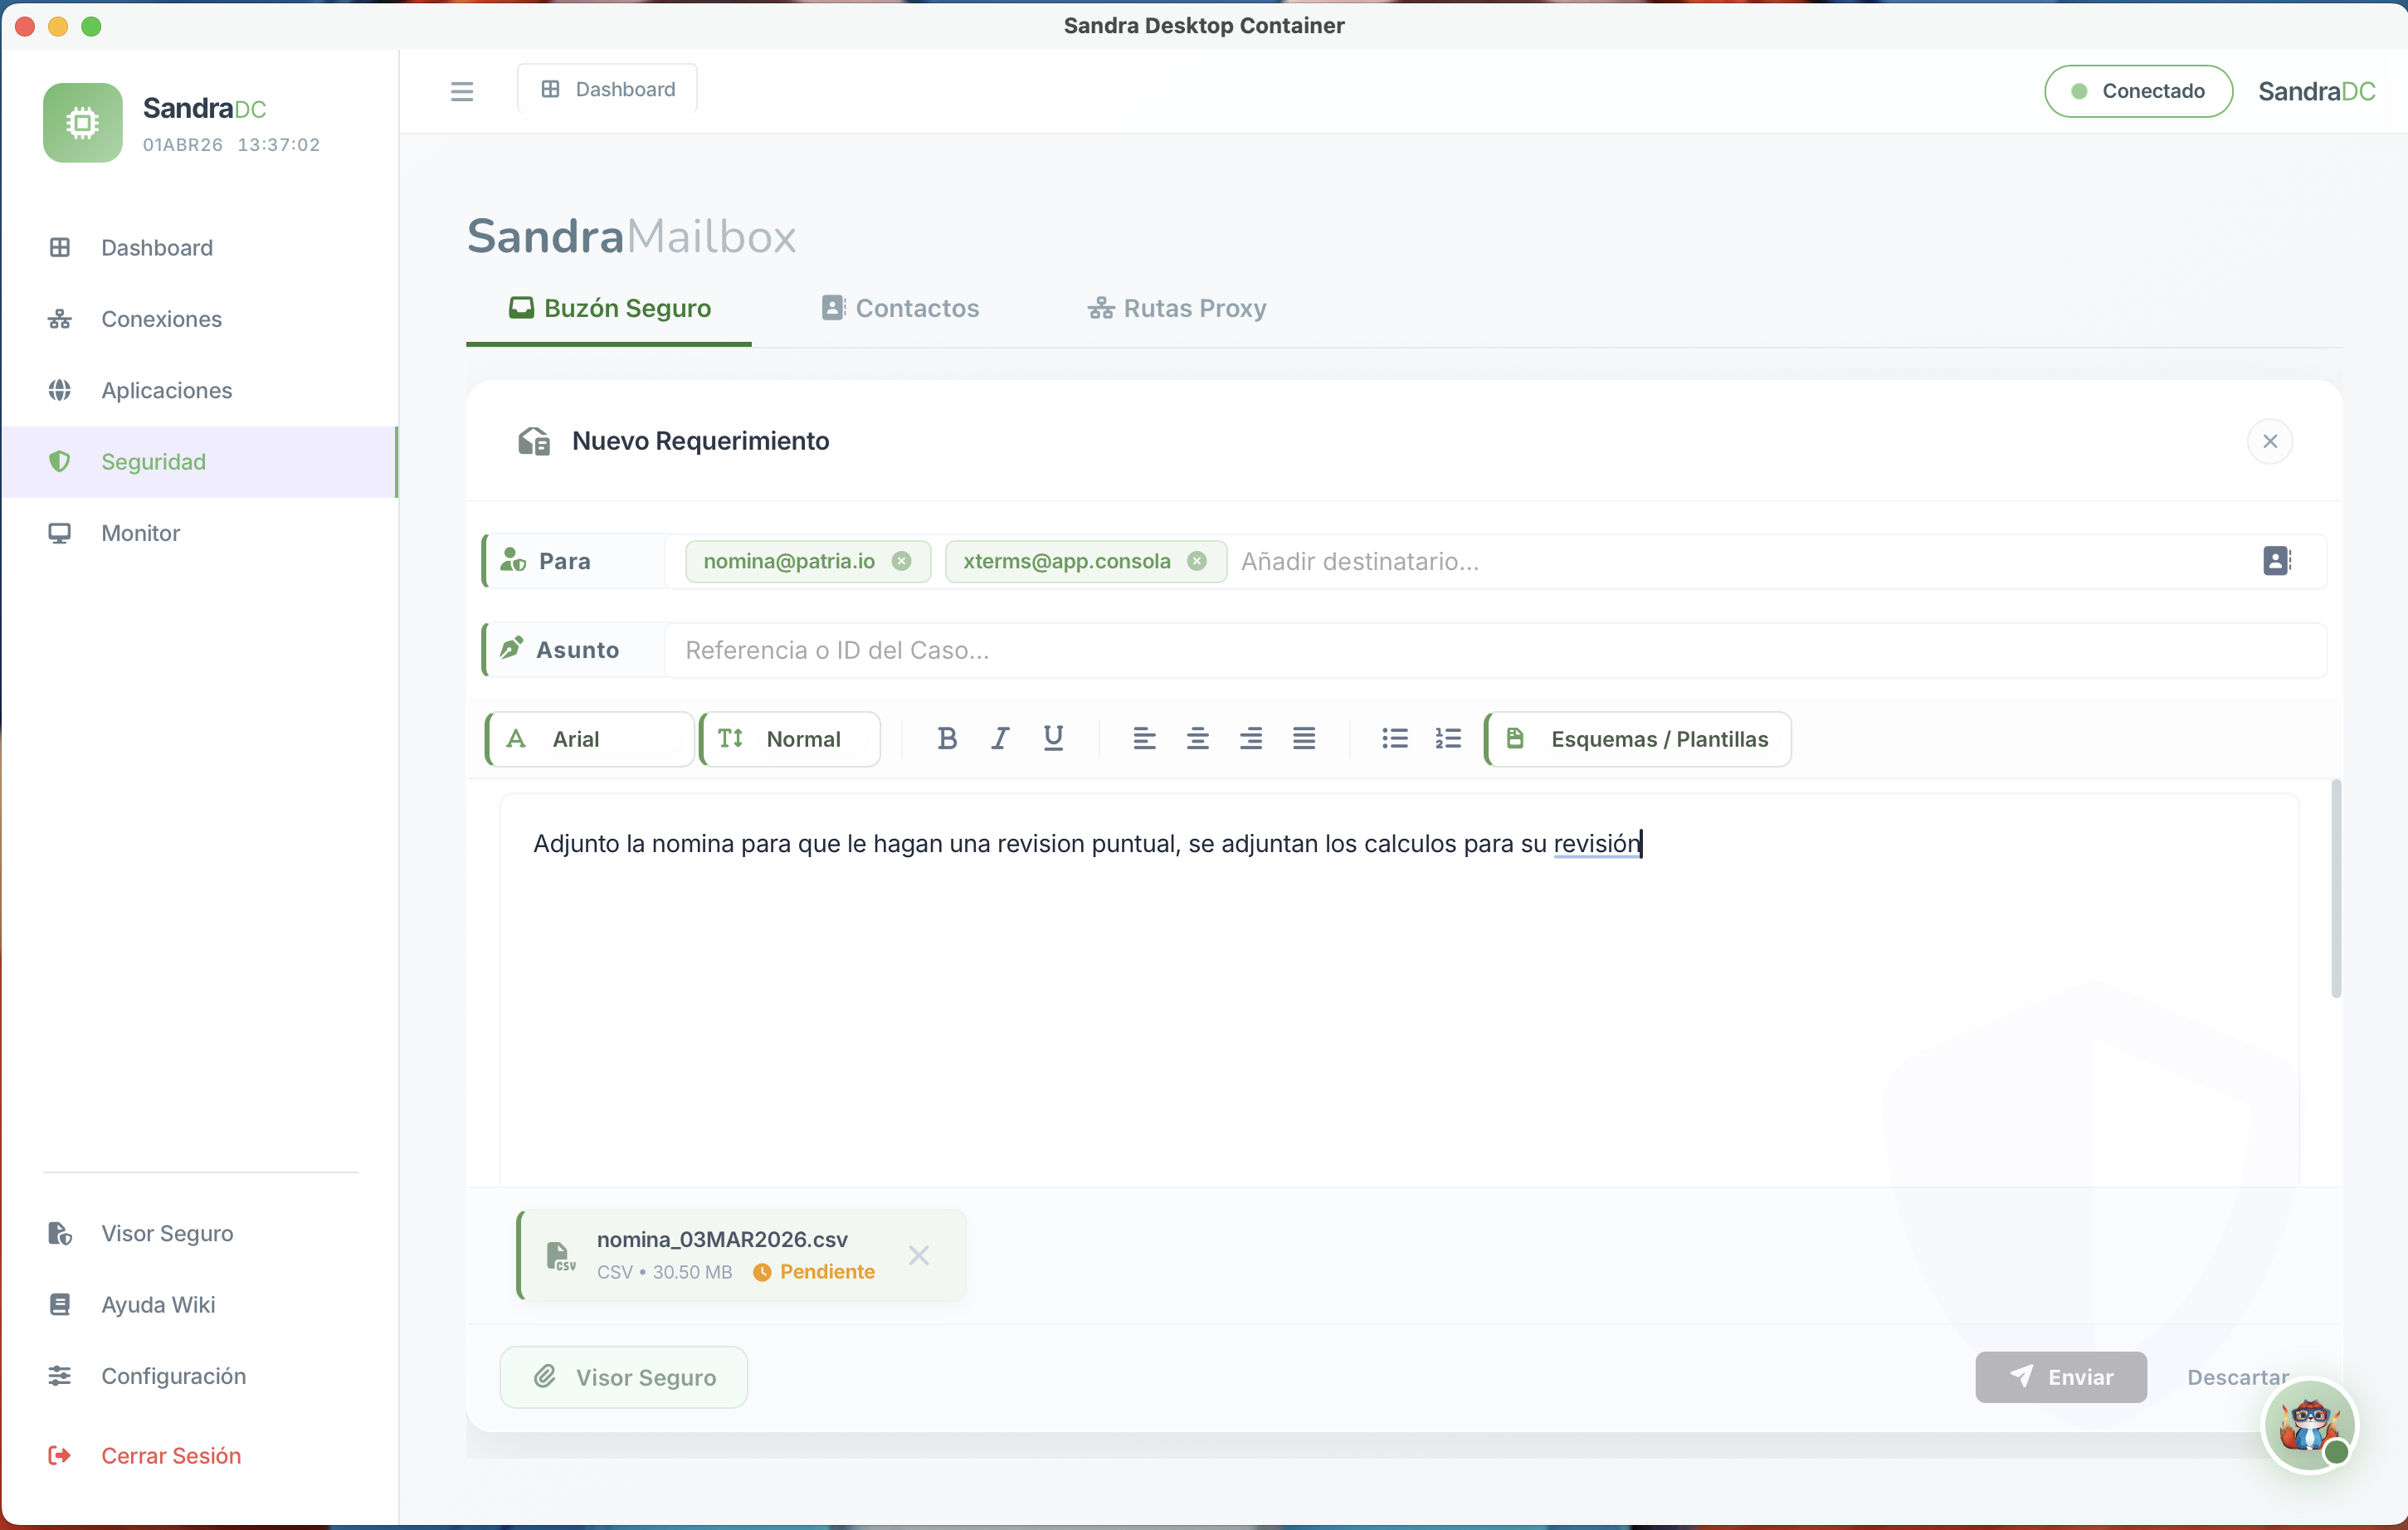
\includegraphics[width=0.95\textwidth]{anexos/7 seguridad.mailbox.nuevo.png}
caption{Formulario de nuevo mensaje seguro}
\label{fig:mailbox-nuevo}
\end{figure}

Al redactar un nuevo mensaje, el usuario cuenta con:

\begin{itemize}[leftmargin=*]
    \item \textbf{Destinatario}: Selector de contactos desde el directorio
    \item \textbf{Asunto}: Campo de texto para identificacion del mensaje
    \item \textbf{Contenido}: Editor de texto con soporte para formato basico
    \item \textbf{Archivos Adjuntos}: Selector de archivos locales para cifrado y envio
    \item \textbf{Importancia}: Indicador de prioridad del mensaje
\end{itemize}

\begin{caja}{Cifrado Automatico}
Todos los mensajes enviados a traves del Buzon de Seguridad son cifrados automaticamente utilizando la clave publica del destinatario y la clave privada del dispositivo emisor, garantizando la confidencialidad del contenido.
\end{caja}

\subsection{Gestion de Archivos Adjuntos}

\begin{figure}[H]
\centering
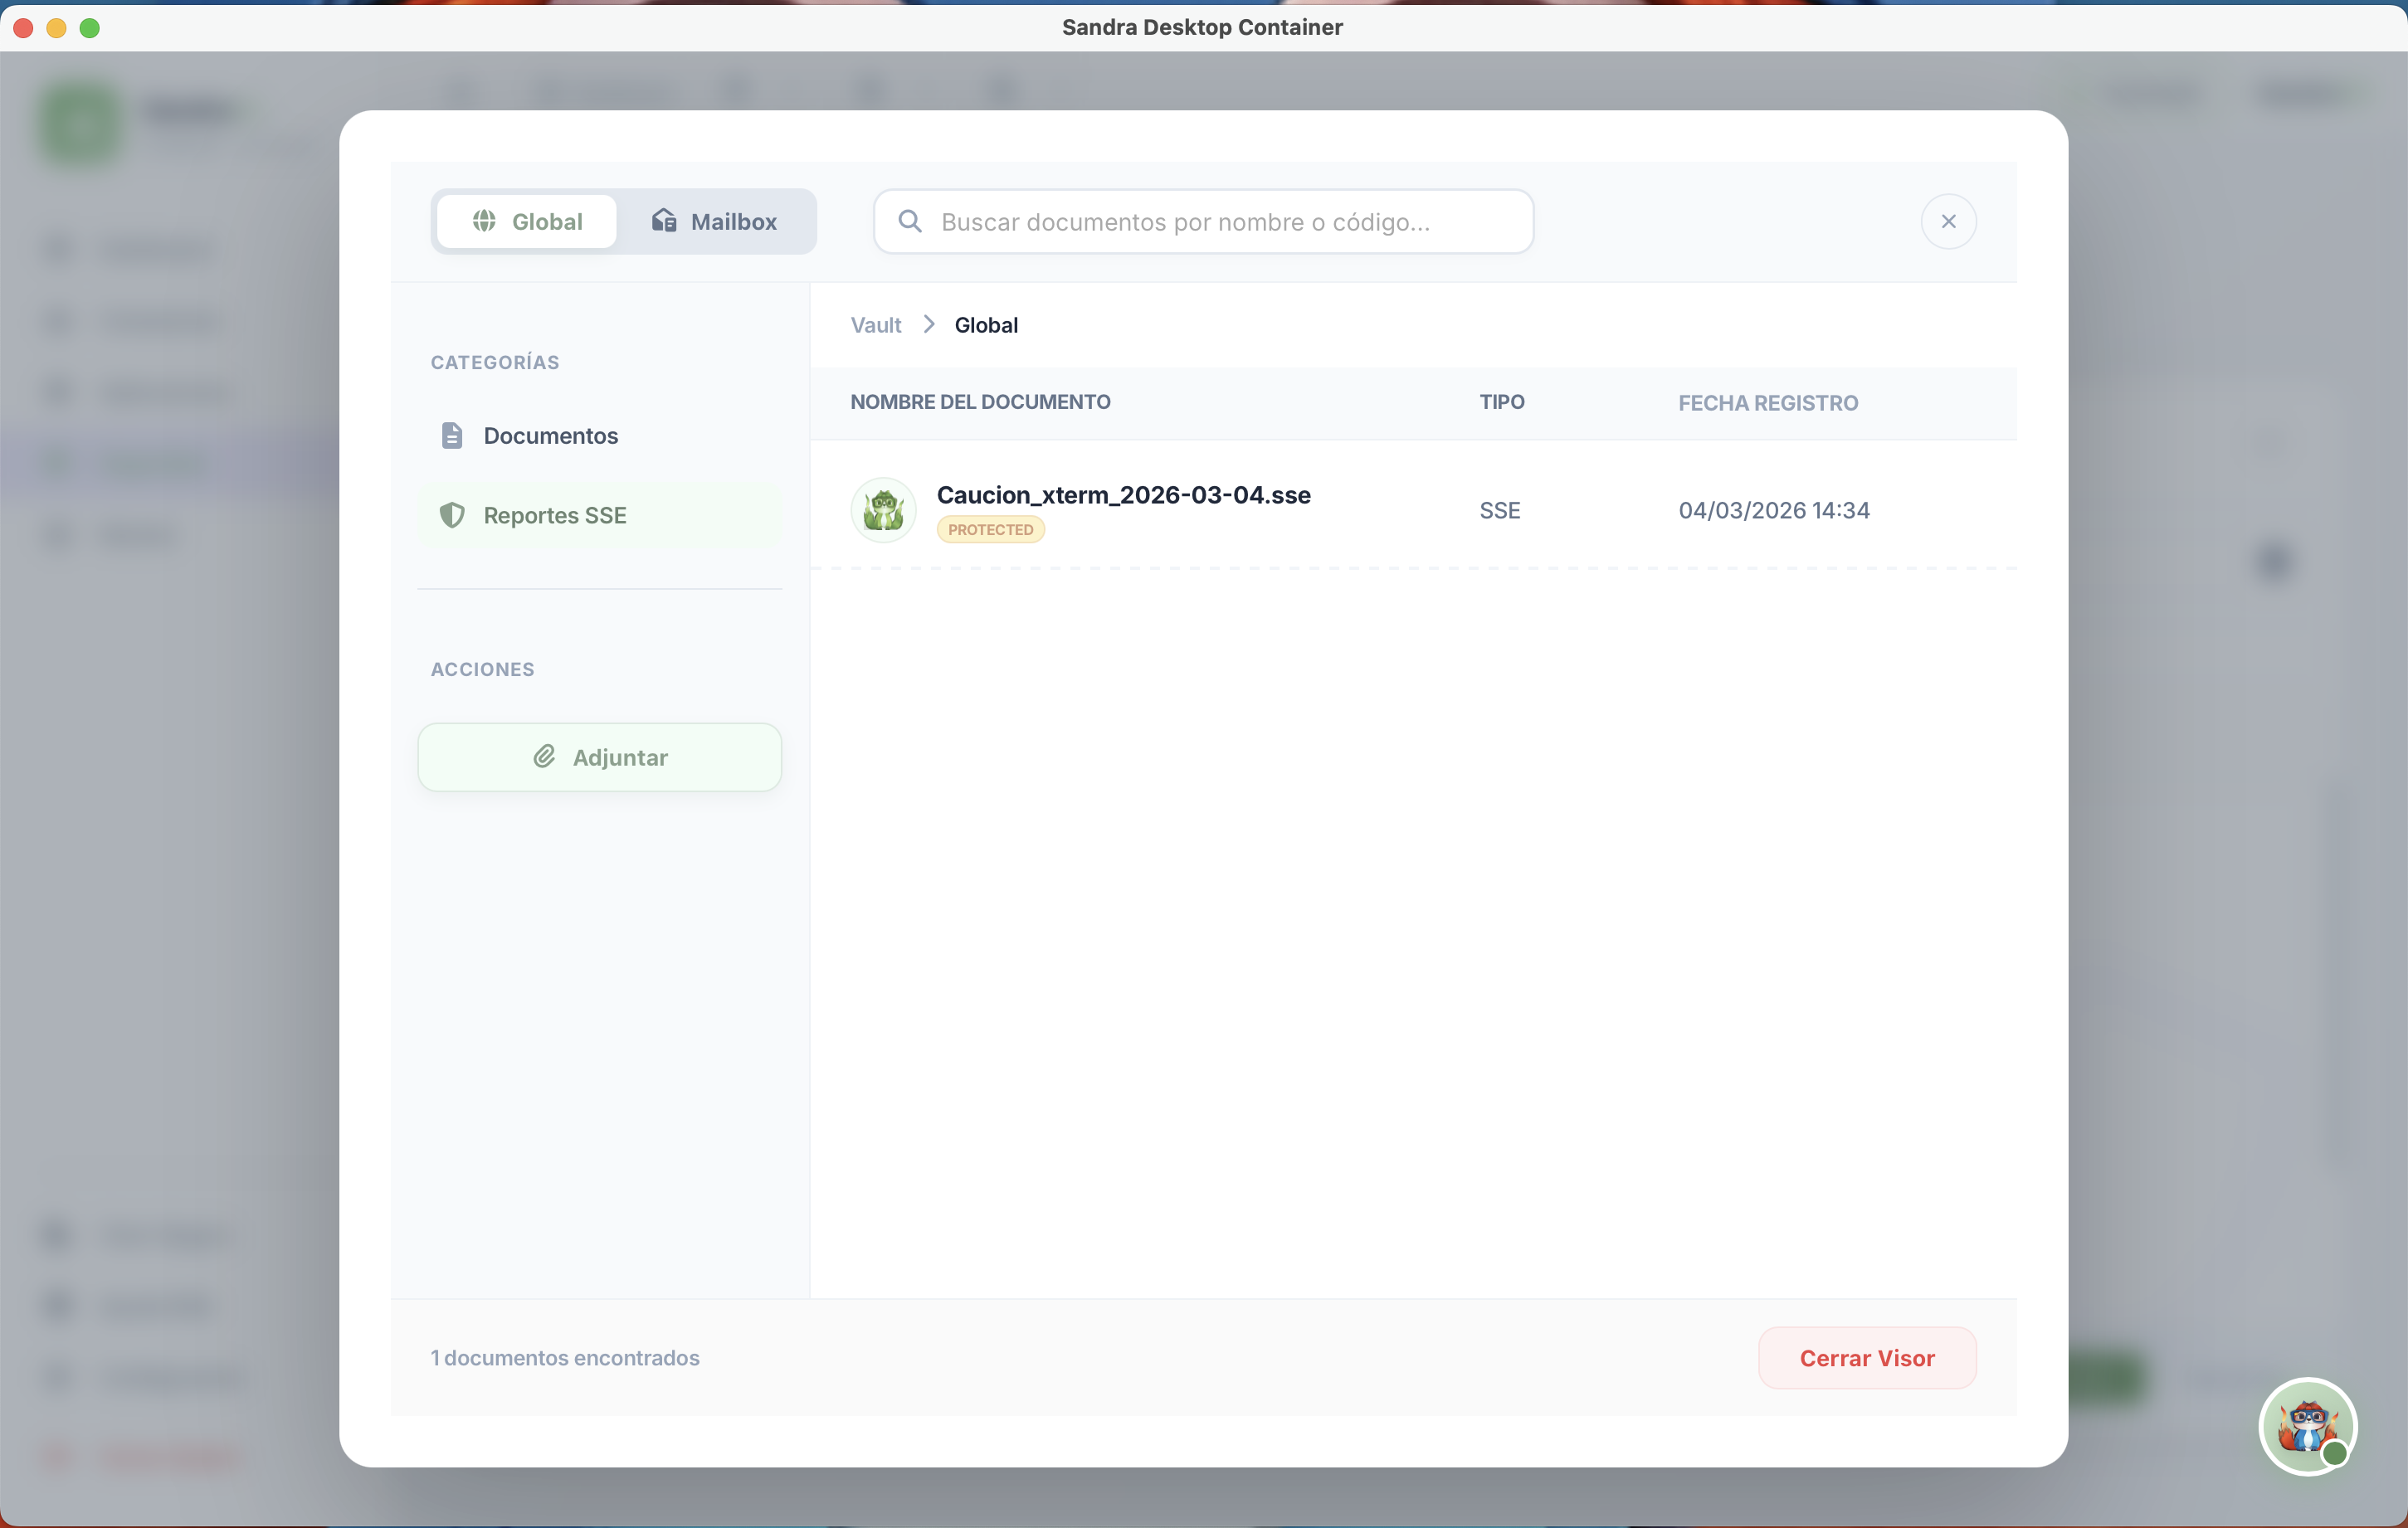
\includegraphics[width=0.95\textwidth]{anexos/7 seguridad.mailbox.nuevo.selector.archivos.png}
caption{Selector de archivos adjuntos}
\label{fig:mailbox-archivos}
\end{figure}

El sistema permite adjuntar archivos que seran:

\begin{enumerate}
    \item \textbf{Cifrados}: Cada archivo se cifra independientemente con AES-256-GCM
    \item \textbf{Empaquetados}: Los archivos se unen en un paquete .sdc (Sandra Secure Container)
    \item \textbf{Verificados}: Se genera un hash SHA-256 para verificacion de integridad
    \item \textbf{Transmitidos}: El paquete se envia mediante el canal seguro WSS
\end{enumerate}

\notacientifica{El formato .sdc permite que los archivos adjuntos sean interoperables con otros dispositivos SDC, incluyendo el mecanismo de Dual-Key Decryption para backward compatibility.}

\notacientifica{Los archivos nunca se almacenan en texto plano en el servidor ni en el cliente. El cifrado es de extremo a extremo.}

\subsection{Notificaciones y Seguimiento}

\begin{figure}[H]
\centering
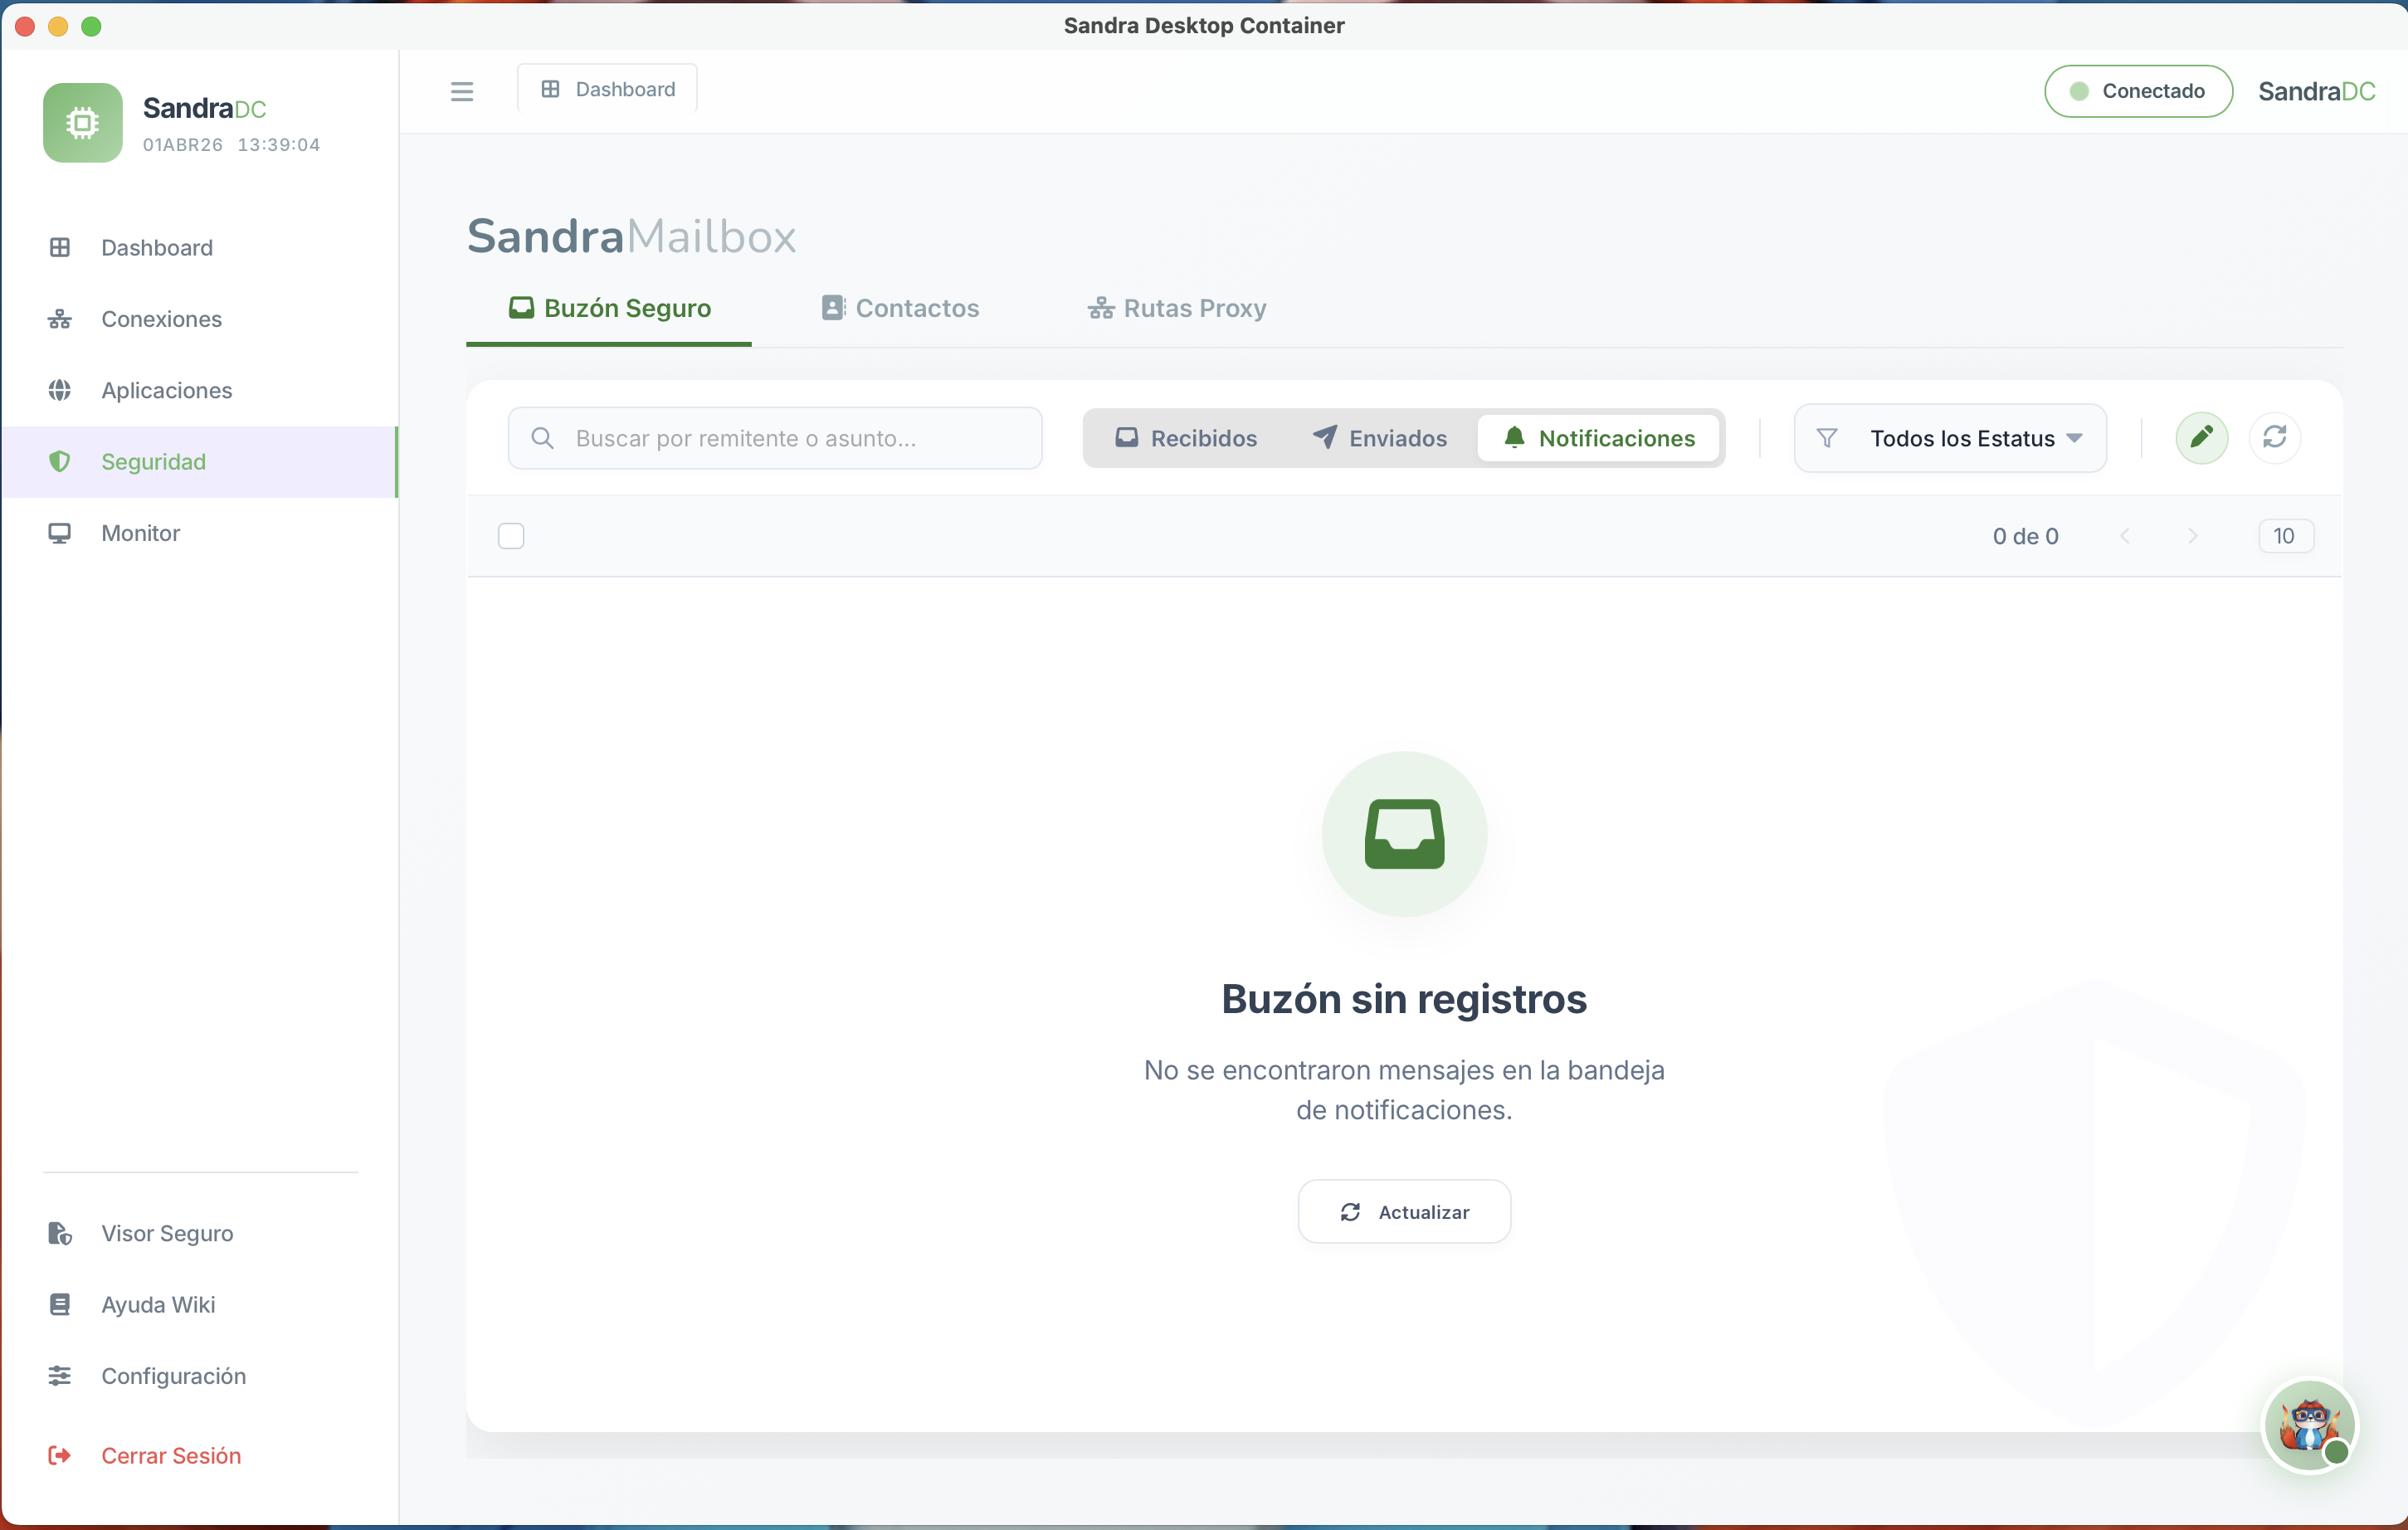
\includegraphics[width=0.95\textwidth]{anexos/7 seguridad.mailbox.notificaciones.png}
caption{Panel de notificaciones del Buzon}
\label{fig:mailbox-notif}
\end{figure}

El sistema de notificaciones proporciona feedback en tiempo real:

\begin{table}[H]
\centering
\begin{tabular}{p{3cm}p{9cm}}
\toprule
\textbf{Estado} & \textbf{Descripcion} \\
\midrule
\cellcolor{sandraGreen} Entregado & Mensaje arrived al servidor del destinatario \\
\midrule
\cellcolor{sandraAccent} Leido & Destinatario abrio el mensaje \\
\midrule
\cellcolor{red!70} Fallido & Error en la entrega, reintento automatico \\
\midrule
\cellcolor{blue!50} Pendiente & Mensaje en cola de envio \\
\bottomrule
\end{tabular}
\caption{Estados de notificacion del Buzon}
\label{tab:notif-estados}
\end{table}

\section{SandraChatBox}
\label{sec:chatbox}

El modulo \keyconcept{SandraChatBox} es el centro de comunicaciones persistente y auditable del contenedor. Ha evolucionado de una simple interfaz de comandos a un sistema completo de mensajeria.

\begin{figure}[H]
\centering
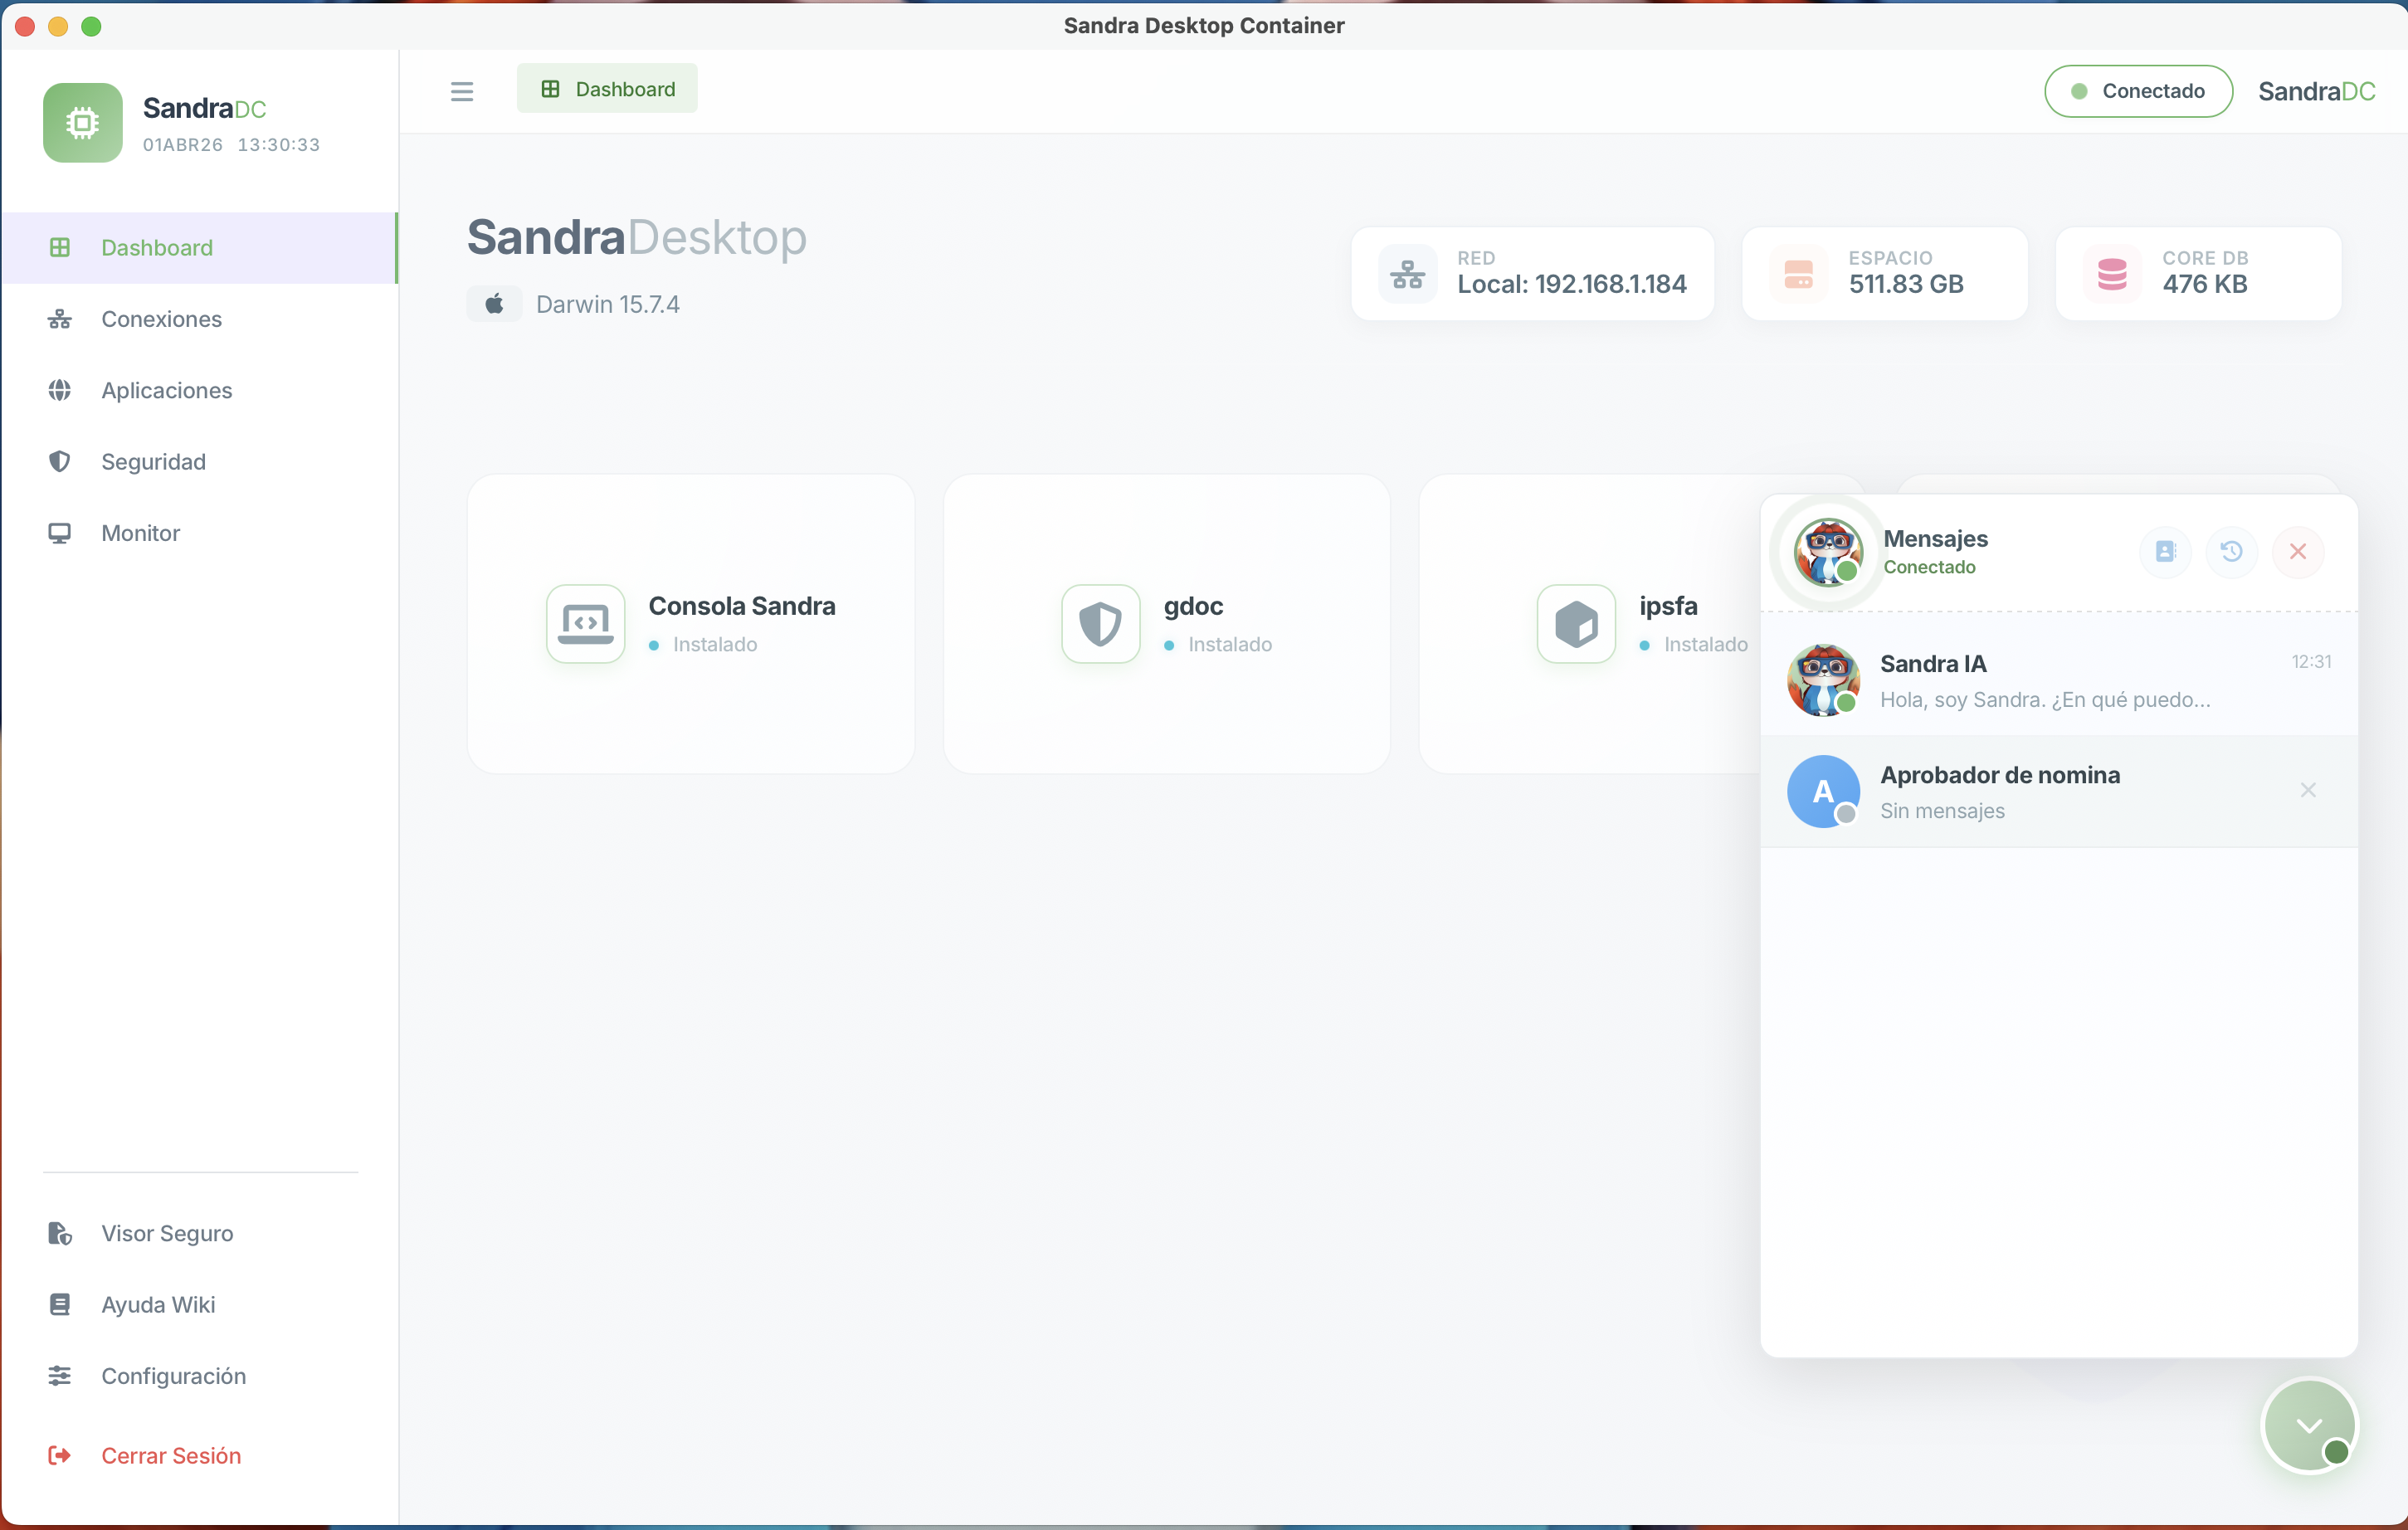
\includegraphics[width=0.65\textwidth]{anexos/22 chat.principal.png}
caption{Interfaz principal de SandraChatBox}
\label{fig:chat-principal}
\end{figure}

\subsection{Gestion de Historial por Sesiones}

El ChatBox implementa un sistema avanzado de gestion del historial:

\begin{caja}{Caracteristicas del Historial}
\begin{itemize}
    \item \textbf{Agrupacion Temporal}: Los mensajes se agrupan automaticamente por fecha, facilitando la lectura de hilos historicos
    \item \textbf{Persistencia de Sesion}: Motor de busqueda y eliminacion selectiva que permite borrar sesiones individuales
    \item \textbf{Borrador Maestro}: Opcion de eliminacion masiva para cumplimiento de protocolos de seguridad post-operacion
    \item \textbf{Scroll Inteligente}: Auto-scroll con deteccion de interaccion del usuario para evitar saltos bruscos durante接收 de rafagas de mensajes
\end{itemize}
\end{caja}

\notacientifica{El sistema de scroll inteligente aprende de los habitos del usuario, ajustando automaticamente la velocidad de desplazamiento para proporcionar una experiencia fluida.}

\subsection{Lista de Conversaciones}

\begin{figure}[H]
\centering
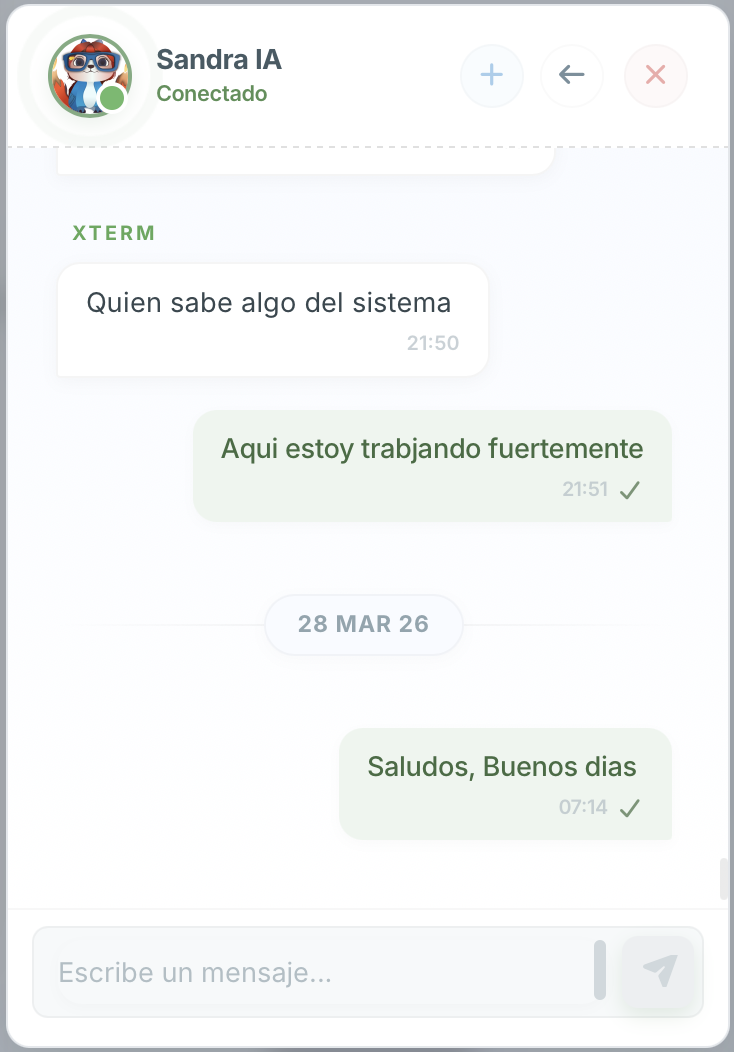
\includegraphics[width=0.65\textwidth]{anexos/22 chat.conversaciones.png}
caption{Lista de conversaciones activas}
\label{fig:chat-conversaciones}
\end{figure}

La vista de conversaciones muestra:

\begin{itemize}[leftmargin=*]
    \item \textbf{Avatar}: Imagen del contacto o iniciales generadas automaticamente
    \item \textbf{Nombre}: Identificador del contacto o grupo
    \item \textbf{Ultimo Mensaje}: Previsualizacion del ultimo mensaje recibido
    \item \textbf{Fecha}: Marca de tiempo relativa (hace X minutos/horas)
    \item \textbf{Indicador}: Icono de no leidos o notificaciones pendientes
\end{itemize}

\notacientifica{Las iniciales se generan con paletas de colores dinamicas basadas en el hash del contacto, permitiendo identificacion rapida sin necesidad de avatar.}

\subsection{Vista de Conversacion}

\begin{figure}[H]
\centering
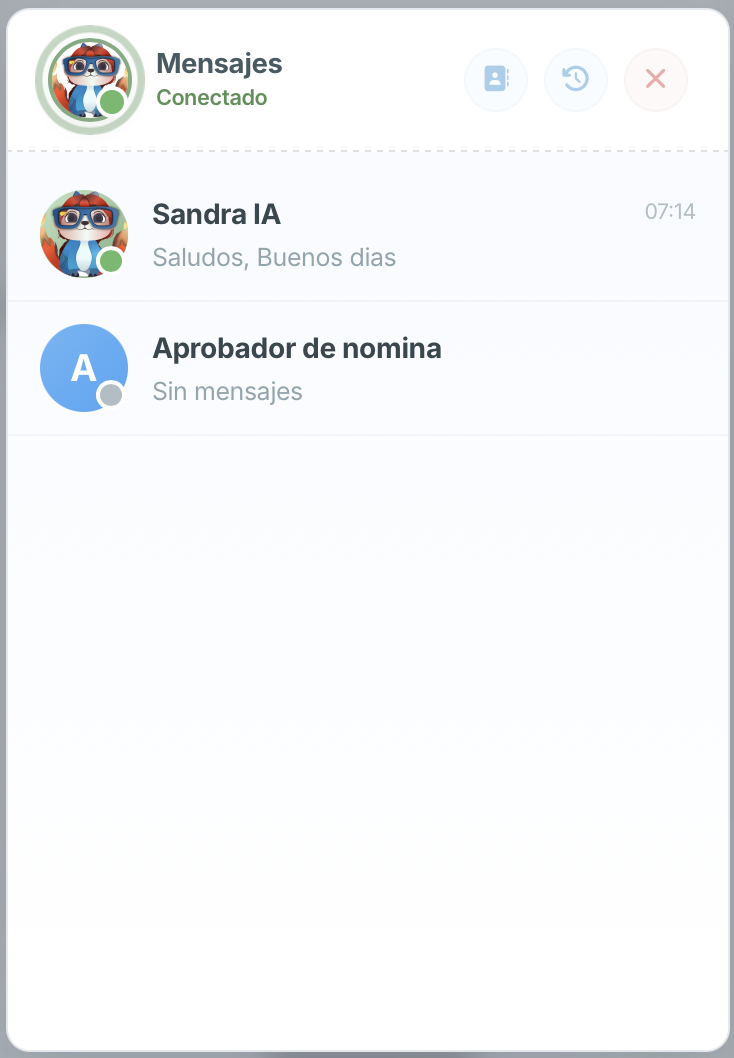
\includegraphics[width=0.65\textwidth]{anexos/22 chat.mensaje.png}
caption{Vista de mensajes en conversacion}
\label{fig:chat-mensaje}
\end{figure}

Cada conversacion muestra:

\begin{enumerate}
    \item \textbf{Header}: Nombre del contacto, estado de conexion, opciones
    \item \textbf{Area de Mensajes}: Historial de mensajes con burbujas diferenciadas (emisor/receptor)
    \item \textbf{Input}: Campo de texto con soporte para envio rapido
    \item \textbf{Indicadores}: Marcas de lectura, hora de envio
\end{enumerate}

\notacientifica{Cada mensaje saliente incorpora automaticamente el perfil del autor (Usuario y Sistema) extrido del JWT de sesion, garantizando que el receptor pueda validar la procedencia del comando.}

\subsection{Agenda de Contactos}

\begin{figure}[H]
\centering
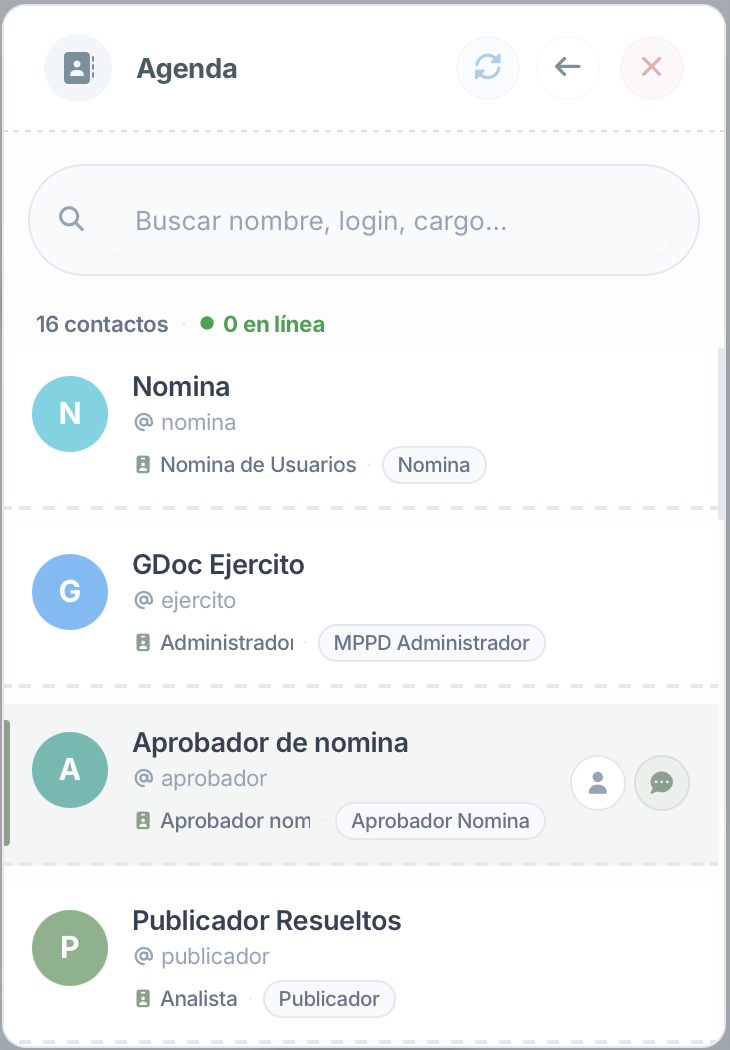
\includegraphics[width=0.65\textwidth]{anexos/22 chat.agenda.png}
caption{Agenda de contactos del chat}
\label{fig:chat-agenda}
\end{figure}

El modulo de agenda permite:

\begin{itemize}[leftmargin=*]
    \item \textbf{Sincronizacion de Directorio}: Recupera el directorio global de usuarios del servidor remoto
    \item \textbf{Contactos Locales}: Gestion de favoritos y contactos frecuentes
    \item \textbf{Busqueda Avanzada}: Filtro en tiempo real por usuario, sistema o identificadores tecnicos
    \item \textbf{Perfiles de Usuario}: Visualizacion de detalles del contacto (nombre, organizacion, clave publica)
\end{itemize}

\notacientifica{La busqueda esta optimizada para responder en menos de 10ms sobre millares de registros, utilizando indices en memoria.}

\subsection{Perfiles y Configuracion}

\begin{figure}[H]
\centering
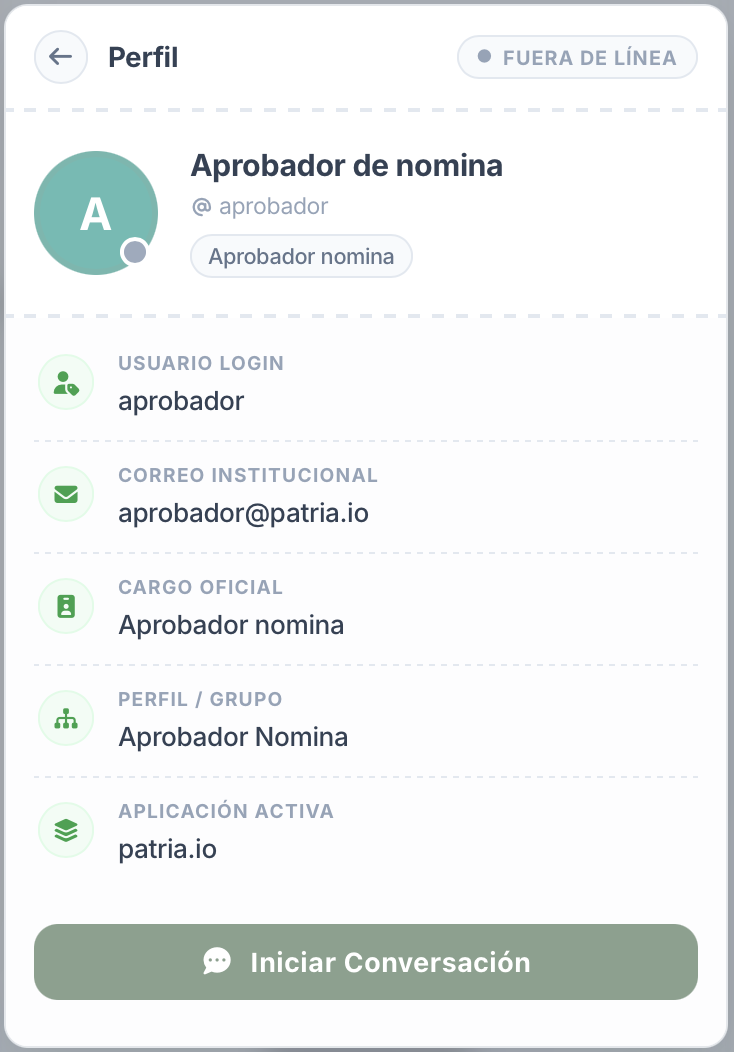
\includegraphics[width=0.65\textwidth]{anexos/22 chat.perfiles.png}
caption{Configuracion de perfiles de usuario}
\label{fig:chat-perfiles}
\end{figure}

Las opciones de perfil incluyen:

\begin{table}[H]
\centering
\begin{tabular}{p{4cm}p{8cm}}
\toprule
\textbf{Opcion} & \textbf{Descripcion} \\
\midrule
Nombre Visible & Nombre que se muestra a otros usuarios \\
\midrule
Estado & Indicador de disponibilidad (Online/Away/Busy) \\
\midrule
Notificaciones & Configuracion de alertas por tipo de mensaje \\
\midrule
Privacidad & Control de quien puede ver el perfil \\
\midrule
Tema & Personalizacion visual del chat \\
\bottomrule
\end{tabular}
\caption{Opciones de configuracion del perfil}
\label{tab:perfil-opciones}
\end{table}

\notacientifica{El sistema de temas permite al usuario personalizar la apariencia del chat, incluyendo colores de burbujas, tipografia y densidad de mensajes.}

\subsection{Eliminacion de Historial}

\begin{figure}[H]
\centering
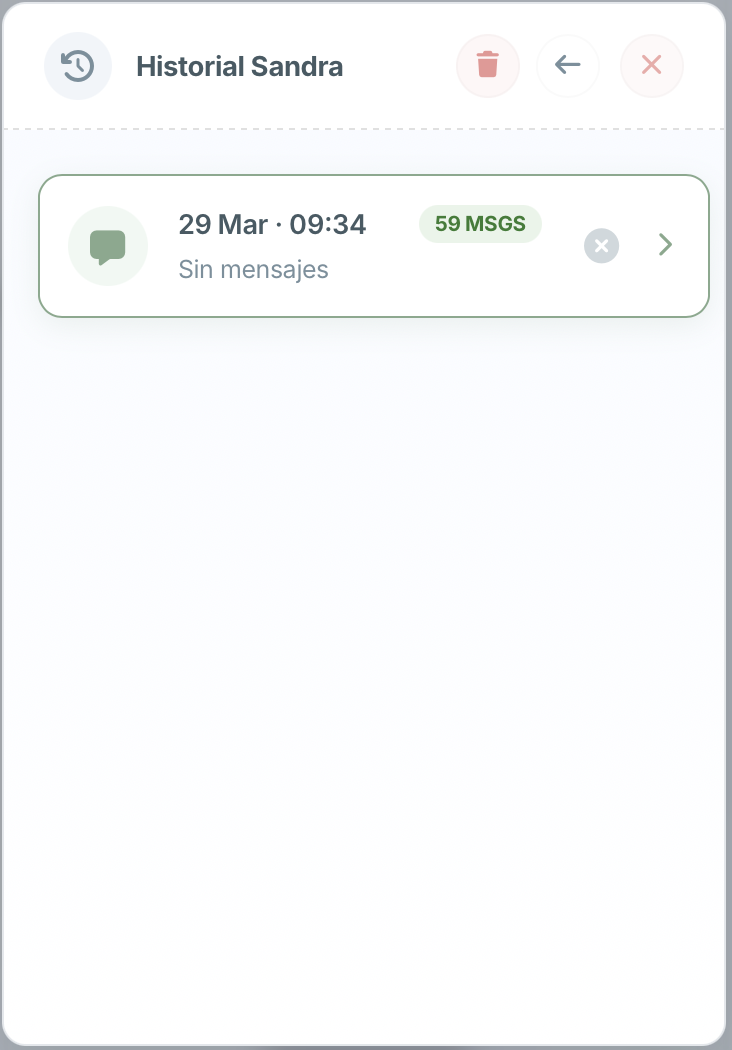
\includegraphics[width=0.65\textwidth]{anexos/22 chat.historial.png}
caption{Opciones de eliminacion de historial}
\label{fig:chat-historial}
\end{figure}

El ChatBox ofrece multiples opciones de eliminacion:

\begin{enumerate}
    \item \textbf{Eliminar Mensaje}: Borra un mensaje especifico de la conversacion
    \item \textbf{Eliminar Conversacion}: Borra toda la conversacion mantiendo el contacto
    \item \textbf{Eliminar Chat Completo}: Borra conversacion y contacto
    \item \textbf{Borrador Maestro}: Eliminacion de todas las conversaciones mayores a X dias
\end{enumerate}

\begin{caja}{Seguridad de Eliminacion}
Al eliminar mensajes o conversaciones, el sistema realiza un borrado seguro que incluye:
\begin{itemize}
    \item Eliminacion de indices de busqueda
    \item Marcado de espacio como disponible en la base de datos
    \item Registro de auditoria del evento de eliminacion
\end{itemize}
Los datos eliminados no pueden ser recuperados por el usuario ni por administradores.
\end{caja}

\notacientifica{El borrado de conversaciones es irreversible y cumple con los protocolos de seguridad post-operacion, generando un log de auditoria para cumplimiento normativo.}

\subsection{Integracion con el Motor de Seguridad}

SandraChatBox esta fuertemente integrado con el sistema de seguridad de SDC:

\begin{caja}{Features de Seguridad del Chat}
\begin{enumerate}
    \item \textbf{Inyeccion de Identidad}: Cada mensaje incorpora el perfil del autor desde el JWT de sesion
    \item \textbf{Filtro de Contenido}: Sanitizacion proactiva de mensajes para prevmir la ejecucion de scripts maliciosos
    \item \textbf{Cifrado de Extremo a Extremo}: Los mensajes se cifran antes de ser enviados
    \item \textbf{Logs de Auditoria}: Toda actividad del chat se registra para auditoria
\end{enumerate}
\end{caja}

\notacientifica{La integracion con el motor de seguridad garantiza que ninguna funcionalidad del chat pueda ser explotada para ataques de-inyeccion de codigo o extraccion de datos no autorizada.}
